
\newpage
\section*{TO DO LIST}
\begin{enumerate}
\item Comparison with other old results on the diode bridge and the buck converter to validate the approach. Otherwise, we suppress the part time's stepping scheme ?
\item Evaluation of the cost of the automatic formualtion
\end{enumerate}
 \newpage
 \section{Aim of this document}
 The goal of this document is a feasibility study to develop an automatic circuit equation
 formulation and software taking into account eventual non smooth components. It consists in including in the standard framework of SPICE piecewise linear laws  and complementarity conditions. The first part studies the modified nodal analysis(M.N.A). As a starttig point, the
 MNA will be used and we will see how it is adapted to manage the non smooth components.
 \section{Notations}
\begin{itemize}
  \item[--] U is a tension, I is a current.
  \item[--] V denotes a potential at node.
  \item[--] q denotes a charge in a capacitor.
  \item[--] $\psi$ denotes a flux in a inductor.
  \item[--] Indice $_{a}$ denotes the current branch.
  \item[--] Indice $_{b}$ denotes the other branch whose voltage is a controlling variable.
  \item[--] Indice $_{c}$ denotes the other branch whose current is a controlling variable.
\item[--] CD : Current Defined
\item[--] VD : Voltage Defined
\item[--] MNA : Modify Nodal Analysis
\item[--] DAE : Differential-Algebraic Equations
\item[--] MLCP : Mixed Linear Complementarity Problem.
\item[--] $N_{I}$ : Number of unknowns.
\item[--] $N_{E}$ : Number of equations.
\item[--] $I_{j}$ : Current in the branch number j.
\item[--] $V_{i}$ : Voltage on node number i.
\end{itemize}

 
\section{Introduction, Modified Nodal Analysis}
This part is a short overview about the Modified Nodal Analysis(MNA). The MNA is the method used
in SPICE to obtain the circuit equation formulation. For more details, we refer the reader to [1][2].%~\cite{Ogrodzki1994,chua1991}.

\subsection{Basics on circuit topology}

Circuits are basically composed of branches, characterized by a current and a related voltage.
Moreover, branches are connected to circuit nodes. The physical behavior of the circuit obeys
Kirchhoff's law. Circuit analysis leads to a mathematical formulation which will be describe in this
document.

\subsubsection{Circuit branches}
\begin{figure}[h]
\centerline{
 \scalebox{0.6}{
    \input{Branch.pstex_t}
 }
}
\caption{Basic branch}
\label{fig-Basic-branch}
\end{figure}
In any case, the branch is described by a pair of branch variables: the tension $U_{a}$ and the current $I_{a}$.
Moreover, the Branch Constitutive Equation can be expressed in a general implicit form:
\begin{equation}\label{BCE}F(U_{a},I_{a},...)=0\end{equation}
We will see the different forms of this relation.
\subsubsection{The Kirchhoff Current Law (KCL)}
\newtheorem{kcl}{Kcl}
\begin{kcl}
At any node in an electrical circuit where charge density is not changing in time, the sum of
currents flowing towards that node is equal to the sum of currents flowing away from that node.
\end{kcl}
The KCL law gives rise to this type of equation:\\
\begin{equation}
 \sum_{i} I_{i}=0\label{eq:KCL}
\end{equation}

\begin{figure}[h]
\centerline{
 \scalebox{0.6}{
    \input{SimpleCircuit.pstex_t}
 }
}
\caption{Circuit and a graph representing its topology}
\label{fig-Circuit-example}
\end{figure}
With the example shown in figure \ref{fig-Circuit-example}, the KCL leads to the following equations:
\[-I_{1}+I_{2}+I_{3}=0\]
\[-I_{3}+I_{4}=0\]
\[I_{1}-I_{2}-I{4}=0\]
or the matrix formulation :
\[AI=0\]
where A is known as the incidence matrix and I is the vector of branch currents.
\subsubsection{The Kirchhoff Voltage Law (KVL)}
\newtheorem{kvl}{Kvl}
\begin{kvl}
The directed sum of the electrical differences around a closed circuit must be zero.
\end{kvl}
With the example shown in figure \ref{fig-Circuit-example}, the KVL leads to the following
equations:
\[U_{1}+U_{2}=0\]
\[-U_{2}+U_{3}+U_{4}=0\]
\[U_{1}+U_{3}+U_{4}=0\]
These equations contain redundancy and the system can be written:
\[\left(\begin{array}{cccc}
  1&1&0&0\\
  0&-1&1&1\\
  \end{array}\right)U=0
  \]
  where U is the vector of tensions. The matrix is known as the loop matrix B.
  \subsubsection{General equations formulation}
  The physical behavior of an electrical circuit can be describe with the following equations:
  \[AI=0\]
  \[BU=0\]
  \[\textrm{For all branches :} \qquad F(U_{a},I_{a},...)=0 \]
\subsection{Definition}
\newtheorem{mur}{Def}
\begin{mur}
The branch is current-defined if its currents is a function of its own voltage, controlling variable
or their time--derivatives:
\begin{equation}\label{CD}I_{a}=F_{i}(U_{a},U_{b},I_{c},\frac{dU_a}{dt},\frac{dU_b}{dt},\frac{dI_{c}}{dt})\end{equation}
\end{mur}
Examples : \\
A resistor is a current-defined branch because $I_{a}=\frac{U_{a}}{R}$.\\
A capacitor is a current-defined branch because $I_{a}=C\frac{dU_{a}}{dt}$.\\
\begin{mur}
The branch is voltage-defined if its voltage is a function of its own current, controlling variable
or their derivatives:
\begin{equation}\label{VD}U_{a}=F_{u}(I_{a},U_{b},I_{c},\frac{dU_a}{dt},\frac{dU_b}{dt},\frac{dI_{c}}{dt})\end{equation}
\end{mur}
Examples : \\
A resistor is a voltage-defined branch because $U_{a}=RI_{a}$.\\
A inductor is a voltage-defined branch because $U_{a}=L\frac{dI_{a}}{dt}$.\\
\subsection{Hypothesis}
The M.N.A. assumes smooth branches are explicit functions of current or voltage. It means each branch is either Voltage Defined (V.D.) or Current Defined (C.D.)\\
\subsection{Unknowns}
The M.N.A. use the following unknowns:
\begin{enumerate}
\item Nodal voltages
\item Currents in the V.D. branches
\item Capacitor's charges and currents
\item Inductor's flux and currents
\item Currents control
\end{enumerate}
These unknowns are the state variables which are assumed to be sufficient to describe the state of the circuit.
\subsection{Equations}
The M.N.A. use following equations:


Current from current-defined branch is replaced with relation~(\ref{CD}). The result is a linear relation between system's unknowns.
\subsubsection{Law in voltage-defined branches (LVD)}
It consists in replacing $U_{a}$ with $V_{i}-V_{j}$ in the relation \ref{VD} and we obtain a linear relation between system's unknowns.
\[V_{i}-V_{j}=F_{i}(I_{a},U_{b},I_{c},\frac{dU_a}{dt},\frac{dU_b}{dt},\frac{dI_{c}}{dt})\]
\subsubsection{Capacitor laws (CAP)}
In a capacitor branch, the voltage is defined by 
\begin{equation}
 q_{a}=CU_{a} 
\end{equation}

A first relation between capacitor charge and nodal tension can be written:\\
\begin{equation}
 q_{a}=C(V_{i}-V_{j})\label{eq:CAP1}\tag{CAP1}
\end{equation}

A second dynamic relation is obtained
\begin{equation}
I_{a}=\frac{dq_{a}}{dt} \label{eq:CAP2}\tag{CAP2}
\end{equation}


After a time discretisation, these equations give to linear relations between system's unknowns.
\subsubsection{Inductor laws (IND)}
A relation between inductor flux and current is defined by
\begin{equation}
\psi _{a}=LI_{a}\label{eq:IND1}\tag{IND1}
\end{equation}
and the  dynamic relation is given by
\begin{equation}
  \label{eq:IND2}
   V_{i}-V_{j}=\frac{d\psi _{a}}{dt} \tag{IND2}
\end{equation}
After a time discretization procedure, these equations give tow linear relations between system's unknowns.
\newpage
\subsection{Stamps method}
The stamps method is an algorithmic method used to fill the table equation from the components. It
consists in writing a sub-table for each type of component, this sub-table is the contribution of the component in the tableau equation.\\
Following, there are stamp examples.
\subsubsection{Resistor stamp}
\[\left(\begin{array}{cccc}
&V_{i}&V_{j}&RSH\\
  \hline
  KCL(i)&\frac{-1}{R}&\frac{1}{R}&\\
  KCL(j)&\frac{1}{R}&\frac{-1}{R}&\\
  \end{array}\right)
\]
Where R is the branch's resistance.
\subsubsection{Conductance stamp}
\[\left(\begin{array}{ccccc}
&V_{i}&V_{j}&I_{a}&RSH\\
  \hline
  KCL(i)&&&1&\\
  KCL(j)&&&-1&\\
  LVD&G&-G&1&\\
  \end{array}\right)
\]
Where G is the branch's conductance.
\subsubsection{Voltage source stamp}
\[\left(\begin{array}{ccccc}
&V_{i}&V_{j}&I_{a}&RSH\\
  \hline
  KCL(i)&&&1\\
  KCL(j)&&&-1\\
  LVD&1&-1&&E
  \end{array}\right)
\]
\subsubsection{Current controlled voltage source stamp}
\[\left(\begin{array}{cccccc}
&V_{i}&V_{j}&I_{a}&I_{b}&RSH\\
  \hline
  KCL(i)&&&1&\\
  KCL(j)&&&-1&\\
  LVD&1&-1&&\gamma
  \end{array}\right)
\]
With $U_{a} = \gamma I_{b}$.
\subsection{General form of the MNA}
The result of the MNA is a system like :
\[MX'=AX+c\]
where X is the vector of unknowns, and M a matrix. Generally, M is not regular. Indeed, some variables
are not dynamic, for example the current in a resistor.
Moreover, If the circuit contains some non-linear components, for example non constant resistors or capacitors,
the matrices M and A will not be constant. In any case, the system can be written as an implicit DAE:
\begin{eqnarray}
F[X,X',t]=0&\label{eq-mna-dae}
\end{eqnarray}

\subsection {Discretization and resolution}

The discretization of the equation ~(\ref{eq-mna-dae}) consists in using the Differentiation Formula
or the Backward Differentiation Formula. It leads to a nonlinear algebraic equation:
\begin{eqnarray}
F[x_{n},z(x_{n},x_{n-1},x_{n-2},...),t_{n}]=0
\end{eqnarray}

This equation is linearized and solved using the Newton-Raphson iterations.

\newpage
\subsection{A simple MNA example}
\begin{figure}[h]
\centerline{
 \scalebox{0.6}{
    \documentclass[10pt]{article}


%% Symbole de fraction
\newcommand{\Frac}[2]{{\displaystyle \frac{\displaystyle #1}{\displaystyle #2}}}
\newcommand{\Prac}[2]{\displaystyle \genfrac{(}{)}{}{}{\displaystyle #1}{\displaystyle #2}}
\newcommand{\Crac}[2]{\displaystyle \genfrac{[}{]}{}{}{\displaystyle #1}{\displaystyle #2}}

\newcommand{\norme}[1]{\|#1\|}


\newcommand{\HRule}{\rule{\linewidth}{1mm}}

% Fonction math�matiques

\newcommand{\transposee}[1]{{\vphantom{#1}}^{\text{\tiny{\textsf T}}}{#1}}
\newcommand{\argmin}{\mathop{\mathrm{argmin}}}
\newcommand{\argminn}{\mathop{\mathrm{argmin}}}
\newcommand{\lexicomin}{\mathop{\mathrm{lexicomin}}}
%\newcommand{\arg}{\mathop{\mathrm{arg}}}



\DeclareMathOperator{\rot}{rot}
\DeclareMathOperator{\sh}{sh}
\DeclareMathOperator{\ch}{ch}
%\DeclareMathOperator{\th}{th}
\DeclareMathOperator{\arcsh}{arcsh}
\DeclareMathOperator{\argth}{argth}
\DeclareMathOperator{\sign}{sign}


%%The Principal Value Integral symbol
\def\Xint#1{\mathchoice
   {\XXint\displaystyle\textstyle{#1}}%
   {\XXint\textstyle\scriptstyle{#1}}%
   {\XXint\scriptstyle\scriptscriptstyle{#1}}%
   {\XXint\scriptscriptstyle\scriptscriptstyle{#1}}%
   \!\int}
\def\XXint#1#2#3{{\setbox0=\hbox{$#1{#2#3}{\int}$}
     \vcenter{\hbox{$#2#3$}}\kern-.5\wd0}}
\def\ddashint{\Xint=}
\def\dashint{\Xint-}



% macro pour les symbols d'ensemble
%\nbOne
\def\nbOne{{\mathchoice{\rm 1\mskip-4mu l}{\rm 1\mskip-4mu l} {\rm 1 \mskip-4.5mu l}{\rm 1\mskip-5mu l}}}
%
%%  Les ensembles de nombres  C. Fiorio (fiorio�at�math.tu-berlin.de) 
%
\def\nbR{\ensuremath{\mathrm{I\!R}}} % IR
\def\nbN{\ensuremath{\mathrm{I\!N}}} % IN
\def\nbF{\ensuremath{\mathrm{I\!F}}} % IF
\def\nbH{\ensuremath{\mathrm{I\!H}}} % IH
\def\nbK{\ensuremath{\mathrm{I\!K}}} % IK
\def\nbL{\ensuremath{\mathrm{I\!L}}} % IL
\def\nbM{\ensuremath{\mathrm{I\!M}}} % IM
\def\nbP{\ensuremath{\mathrm{I\!P}}} % IP
%
% \nbOne : 1I : symbol one
\def\nbOne{{\mathchoice {\rm 1\mskip-4mu l} {\rm 1\mskip-4mu l}
{\rm 1\mskip-4.5mu l} {\rm 1\mskip-5mu l}}}
%
% \nbC   :  Nombres Complexes
\def\nbC{{\mathchoice {\setbox0=\hbox{$\displaystyle\rm C$}%
\hbox{\hbox to0pt{\kern0.4\wd0\vrule height0.9\ht0\hss}\box0}}
{\setbox0=\hbox{$\textstyle\rm C$}\hbox{\hbox
to0pt{\kern0.4\wd0\vrule height0.9\ht0\hss}\box0}}
{\setbox0=\hbox{$\scriptstyle\rm C$}\hbox{\hbox
to0pt{\kern0.4\wd0\vrule height0.9\ht0\hss}\box0}}
{\setbox0=\hbox{$\scriptscriptstyle\rm C$}\hbox{\hbox
to0pt{\kern0.4\wd0\vrule height0.9\ht0\hss}\box0}}}}
%
% \nbQ   : Nombres Rationnels Q
\def\nbQ{{\mathchoice {\setbox0=\hbox{$\displaystyle\rm
Q$}\hbox{\raise
0.15\ht0\hbox to0pt{\kern0.4\wd0\vrule height0.8\ht0\hss}\box0}}
{\setbox0=\hbox{$\textstyle\rm Q$}\hbox{\raise
0.15\ht0\hbox to0pt{\kern0.4\wd0\vrule height0.8\ht0\hss}\box0}}
{\setbox0=\hbox{$\scriptstyle\rm Q$}\hbox{\raise
0.15\ht0\hbox to0pt{\kern0.4\wd0\vrule height0.7\ht0\hss}\box0}}
{\setbox0=\hbox{$\scriptscriptstyle\rm Q$}\hbox{\raise
0.15\ht0\hbox to0pt{\kern0.4\wd0\vrule height0.7\ht0\hss}\box0}}}}
%
% \nbT   : T
\def\nbT{{\mathchoice {\setbox0=\hbox{$\displaystyle\rm
T$}\hbox{\hbox to0pt{\kern0.3\wd0\vrule height0.9\ht0\hss}\box0}}
{\setbox0=\hbox{$\textstyle\rm T$}\hbox{\hbox
to0pt{\kern0.3\wd0\vrule height0.9\ht0\hss}\box0}}
{\setbox0=\hbox{$\scriptstyle\rm T$}\hbox{\hbox
to0pt{\kern0.3\wd0\vrule height0.9\ht0\hss}\box0}}
{\setbox0=\hbox{$\scriptscriptstyle\rm T$}\hbox{\hbox
to0pt{\kern0.3\wd0\vrule height0.9\ht0\hss}\box0}}}}
%
% \nbS   : S
\def\nbS{{\mathchoice
{\setbox0=\hbox{$\displaystyle     \rm S$}\hbox{\raise0.5\ht0%
\hbox to0pt{\kern0.35\wd0\vrule height0.45\ht0\hss}\hbox
to0pt{\kern0.55\wd0\vrule height0.5\ht0\hss}\box0}}
{\setbox0=\hbox{$\textstyle        \rm S$}\hbox{\raise0.5\ht0%
\hbox to0pt{\kern0.35\wd0\vrule height0.45\ht0\hss}\hbox
to0pt{\kern0.55\wd0\vrule height0.5\ht0\hss}\box0}}
{\setbox0=\hbox{$\scriptstyle      \rm S$}\hbox{\raise0.5\ht0%
\hboxto0pt{\kern0.35\wd0\vrule height0.45\ht0\hss}\raise0.05\ht0%
\hbox to0pt{\kern0.5\wd0\vrule height0.45\ht0\hss}\box0}}
{\setbox0=\hbox{$\scriptscriptstyle\rm S$}\hbox{\raise0.5\ht0%
\hboxto0pt{\kern0.4\wd0\vrule height0.45\ht0\hss}\raise0.05\ht0%
\hbox to0pt{\kern0.55\wd0\vrule height0.45\ht0\hss}\box0}}}}
%
% \nbZ   : Entiers Relatifs Z
\def\nbZ{{\mathchoice {\hbox{$\sf\textstyle Z\kern-0.4em Z$}}
{\hbox{$\sf\textstyle Z\kern-0.4em Z$}}
{\hbox{$\sf\scriptstyle Z\kern-0.3em Z$}}
{\hbox{$\sf\scriptscriptstyle Z\kern-0.2em Z$}}}}
%%%% fin macro %%%%



\newcommand{\putidx}[1]{\index{#1}\textit{#1}}
% macro pour r�f�rencer les �quations

\newcommand{\refeq}[1]{(\ref{#1})}
\newcommand{\reffig}[1]{({\it cf} figure : \ref{#1})}
\newcommand{\refann}[1]{({\it cf} Annexe : \ref{#1})}


%\definecolor{darkgray}{gray}{.25}
%\definecolor{gray}{gray}{.5}
%\definecolor{lightgray}{gray}{.75}
%\definecolor{gradbegin}{rgb}{0,1,1}
%\definecolor{gradend}{rgb}{0,.1,.95}
%\newcommand{\newtexte}[1]{\textcolor{darkgray} {#1}}
\newcommand{\newtexte}[1]{{#1}}% macro pour les varibales favorites
% normal tangent
\def\n{{\hbox{\tiny{N}}}}
\def\t{{\hbox{\tiny{T}}}}
\def\ss{{\hbox{\tiny{S}}}}
\def\nt{\hbox{\tiny{NT}}}
\def\nsf{\hbox{\tiny{\textsf N}}}
\def\tsf{\hbox{\tiny{\textsf T}}}
\def\sigman{\sigma_{\n}}
\def\sigmat{\sigma_{\t}}
\def\sigmant{\sigma_{\nt}}
\def\epsn{\epsilon_{\n}}
\def\epst{\epsilon_{\t}}
\def\epsnt{\epsilon_{\nt}}
\def\eps{\epsilon}
\def\veps{\varepsilon}
\def\sig{\sigma}
\def\Rn{R_{\n}}
\def\Rt{R_{\t}}
\def\cn{c_{\n}}
\def\Cn{C_{\n}}
\def\ct{c_{\t}}
\def\Ct{C_{\t}}
\def\un{u_{\n}}
\def\ut{\buu_{\t}}
\def\uut{u_{\t}}
\def\unc{u_{\n}^c}
\def\utc{\buu_{\t}^c}
\def\vn{v_{\n}}
\def\vt{v_{\t}}
\def\rr{\hbox{\tiny{\textsf R}}}
\def\irr{\hbox{\tiny{\textsf{IR}}}}
\def\rn{r_{\n}}
\def\rt{\brr_{\t}}
\def\rnc{r_{\n}^c}
\def\rtc{\brr_{\t}^c}
\def\trn{\Tilde{r}_{\n}}
\def\trt{\Tilde{\brr}_{\t}}
\def\tr{\Tilde{\brr}}
\def\tv{\Tilde{\bvv}}
\def\vn{v_{\n}}
\def\vt{\bvv_{\t}}
\def\adh{\mathsf{adh}}
\def\adj{\hbox{\tiny{\textsf{adj}}}}
\def\adjc{\hbox{\tiny{\textsf{adjC}}}}
\def\adja{\hbox{\tiny{\textsf{adjA}}}}
\def\cc{\hbox{\tiny{\textsf C}}}
\def\ca{\hbox{\tiny{\textsf A}}}
%%    Unit�e
\def\mm{\,\mathsf{mm}}
\def\cm{\,\mathsf{cm}}
\def\m{\,\mathsf{m}}
\def\ms{\,\mathsf{m.s^{-1}}}
\def\mms{\,\mathsf{mm.s^{-1}}}
\def\Mpa{\,\mathsf{MPa}}
\def\Gpa{\,\mathsf{GPa}}
\def\Kg{\,\mathsf{Kg}}
\def\Hz{\,\mathsf{Hz}}
\def\kHz{\,\mathsf{kHz}}
\def\N{\,\mathsf{N}}
\def\kN{\,\mathsf{kN}}
\def\Nmmm{\,\mathsf{N.m^{-3}}}
\def\ds{d_{\hbox{\tiny{S}}}}
% domaines et frontieres
\def\om{\Omega}
\def\oma{\Omega^{\alpha}}
\def\omu{\Omega^1\cup \Omega^2}
\def\gc{\Gamma_c}
\def\omt{\omu \cup \gc}
% derivee partielle et gradient et divergence
\def\p{\partial}
\def\grad{\nabla}
\def\div{\mathop{\rm div}\nolimits}
%

%\DeclareTextSymbol{\deg}{T1}{6}
%\def\degre{\mathdegree}
%\newcommand{\degre}{\mathdegree}

\def\etc{\textit{etc}\ldots}
\newcommand{\mdegre}{\hbox{\text{\degre}}}

%\def\nscd{\textsf{\bfseries NSCD}}
%\def\nscd{\textsf{NSCD}}
\newcommand{\nscd}{\textsf{NSCD}}
%\Pisymbol{psy}{212} ou encore \Pisymbol{psy}{228}




%----------------------------------------------------------------------
%             Des chiffres avec des ronds autour
%----------------------------------------------------------------------
\def\nombrecercle#1{\def\taille{0.3}
                \put(0,0){#1}
                \put(0.08,0.08){\circle{\taille}}}



\def\ae#1{\stackrel{\mbox{\scriptsize a.e.}}{#1}}
\def\argmin{\mathop{\rm argmin}}
\def\eqref#1{{\rm (\ref{#1})\/}}
\def\indicfon{\mathord{\rm i}}       %indicator function
\def\p{\mathord{\rm proj}}
\def\N{\mathord{\rm N}}
% \def\prosca#1#2{#1\cdot#2}
\def\prosca#1#2{\langle #1,#2\rangle}
\def\qedtext{\mbox{}\hfill$\Box$}
\def\qedmath{\eqno\Box}

\def\s{{$\mathcal{S}$}}
\def\somme{\mathop{\textstyle\sum}}
\def\somme{\mathop{\textstyle\sum}}
\def\submoins{_{\scriptscriptstyle-}}
\def\subplus{_{\scriptscriptstyle+}}
\def\T{\mathord{\rm T}}

%----------------------------------------------------------------------
%             Macro M Jean 
%----------------------------------------------------------------------

\def\Real{\mbox{I\hspace{-.15em}R}}
\def\Integer{\mbox{I\hspace{-.15em}N}}
\def\Bunit{\mbox{I\hspace{-.15em}B}}
\def\real{\mbox{\scriptsize I\hspace{-.15em}R}}
\def\bunit{\mbox{\scriptsize I\hspace{-.15em}B}}
\def\IL{\mbox{\scriptsize I\hspace{-.15em}L}}
\def\Indic{\mbox{\large $\psi$}}
\def\bfxi{\mbox{$\xi$ \hspace{-1.1em} $\xi$}}
%\def\bfXi{\mbox{$\Xi$ \hspace{-1.1em} $\Xi$}}
\def\RunR{\mathcal R}
\def\RunRN{\mathcal R_{N}}
\def\RunRT{\mathcal R_{T}}
\def\RunS{\mathcal S}
\def\RunSN{\mathcal S_{N}}
\def\RunST{\mathcal S_{T}}
\def\RunU{\mathcal U}
\def\RunUN{\mathcal U_{N}}
\def\RunUT{\mathcal U_{T}}
\def\RunUP{\mathcal U'}
\def\RunUPN{\mathcal U'_{N}}
\def\RunUPT{\mathcal U'_{T}}
\def\RunJ{\mathcal J}
\def\RunW{\mathcal W}
\def\RunF{f}
\def\RunFa{f_{1}}
\def\RunFb{f_{2}}
\def\RunFP{f'}
\def\RunV{v}
\def\RunVP{v'}
\def\EspF{\mathcal F}
\def\EspV{\mathcal V}
%%%%
\catcode`\�=13
\def�{\'e}
\catcode`\�=13
\def�{\`e}
\catcode`\�=13
\def�{\`a}
\catcode`\�=13
\def�{\c c}
\def\N{\mbox{I\hspace{ -.15em}N}}
\def\Z{\mbox{Z\hspace{ -.3em}Z}}
\def\Q{\mbox{l\hspace{ -.47em}Q}}
\def\R{\mbox{l\hspace{ -.15em}R}}
\def\F{\mbox{l\hspace{ -.15em}F}}
\def\E{\mbox{l\hspace{ -.15em}E}}
\def\LMGC90{{\small \it LMGC90 }}
\def\NSCD{{\small \it NSCD }}
\def\CHIC{{\small \it CHIC }}
\def\half{{\frac{_{1}}{^{2}}}}
\def\12T{{\frac{_{1}}{^{2T}}}}

\def\geq{\geqslant}
\def\leq{\leqslant}
\def\ge{\geqslant}
\def\le{\leqslant}


\begingroup
\count0=\time \divide\count0by60 % Hour
\count2=\count0 \multiply\count2by-60 \advance\count2by\time
% Min
\def\2#1{\ifnum#1<10 0\fi\the#1}
\xdef\isodayandtime{\the\year-\2\month-\2\day\space\2{\count0}:%
\2{\count2}}
\endgroup

%---------------------------------------------------------------------
%             Redaction note environnement B. Brogliato
%----------------------------------------------------------------------
\makeatletter

{\newtheorem{ndr1bb}{\textbf{\textsc{Redaction note B.B.}}}[section]}

\newenvironment{ndrbb}%
{%
\noindent\begin{ndr1bb}\hrule\vspace{1em}%
\ttfamily\small
}%
{%
\begin{flushright}%
%\vspace{-1.5em}\ding{111}
\end{flushright}%
\vspace{-1.5em}\hrule
\end{ndr1bb}%
}

%---------------------------------------------------------------------
%             Redaction note environnement O. Bonnefon
%----------------------------------------------------------------------

{\newtheorem{ndr1ob}{\textbf{\textsc{Redaction note O.B.}}}[section]}

\newenvironment{ndrob}%
{%
\noindent\begin{ndr1ob}\hrule\vspace{1em}%
\ttfamily\small
}%
{%
\begin{flushright}%
%\vspace{-1.5em}\ding{111}
\end{flushright}%
\vspace{-1.5em}\hrule
\end{ndr1ob}%
}

%----------------------------------------------------------------------
%             Redaction note environnement V.ACARY
%----------------------------------------------------------------------
% Faut etre fou pour s'amuser a pondre des notes pareilles

{\newtheorem{ndr1va}{\textbf{\textsc{Redaction note V.A.}}}[section]}

\newenvironment{ndrva}%
{%
\noindent\begin{ndr1va}\hrule\vspace{1em}%
\ttfamily\small \  \\
\indent}%
{%
\begin{flushright}%
\  \\
%\vspace{-1.5em}\ding{111}
\end{flushright}%
\vspace{-1.5em}\hrule
\end{ndr1va}%
}
\makeatother






% ----------------DEFINITIONS-----------------
% 

 \def\II{\mathop{{\rm I}\mskip-3.0mu{\rm I}}\nolimits}




% -----------------------------------
 \def\c{\mathop{{\rm 1}\mskip-10.0mu{\rm C}}\nolimits}
 \def\C{\mathop{{\rm 1}\mskip-10.0mu{\rm C}}\nolimits}
 \def\ZZ{\mathaccent23Z}
% 
 \def\abstract{
 \footnotesize\quotation \noindent {\bf Abstract.}}
% 

\newcommand{\ie}{{\textit{i.e.}}}


%\def\sgn{\mbox{\rm sgn}}
\DeclareMathOperator{\sgn}{sgn}
\DeclareMathOperator{\proj}{proj}

\newcommand{\RR}{\mbox{\rm $I\!\!R$}}
\newcommand{\NN}{\mbox{\rm $I\!\!N$}}



% ---------------- MMC -----------------
% 

\newcommand{\contract}{{\,:\,}}

\newcommand{\scontract}{{\,{\Bar\otimes}\,}}
\newcommand{\tcontract}{{\,{\Bar{\Bar{\Bar\otimes}}}\,}}


\newcommand{\DP}[2]{\displaystyle \frac{\partial {#1}}{\partial {#2}}}


\usepackage{pifont}
\makeatletter
\def\cqfd{\ifmmode\sqw\else{\ifhmode\unskip\fi\nobreak\hfil
\penalty50\hskip1em\null\nobreak\hfil\ding{111}
\parfillskip=0pt\finalhyphendemerits=0\endgraf}\fi}
\makeatother
\def\off{{\hbox{\tiny{\textsf{off}}}}}
\def\on{{\hbox{\tiny{\textsf{on}}}}}
\def\pwl{{\hbox{\tiny{\textsf{pwl}}}}}

%%% Local Variables: 
%%% mode: latex
%%% TeX-master: "book"
%%% x-symbol-coding: iso-8859-2
%%% End: 

\usepackage{psfrag}
\usepackage{fancyhdr}
\usepackage{subfigure}
%\renewcommand{\baselinestretch}{1.2}
\textheight 23cm
\textwidth 16cm
\topmargin 0cm
%\evensidemargin 0cm
\oddsidemargin 0cm
\evensidemargin 0cm
\usepackage{layout}
\usepackage{mathpple}
\makeatletter
\renewcommand\bibsection{\paragraph{References
     \@mkboth{\MakeUppercase{\bibname}}{\MakeUppercase{\bibname}}}}
\makeatother
%% style des entetes et des pieds de page
\fancyhf{} % nettoie le entetes et les pieds
\fancyhead[L]{Template 6 : Electrical oscillator with 4 diodes bridge full-wave rectifier - Pascal Denoyelle}
%\fancyhead[C]{}%
\fancyhead[R]{\thepage}
%\fancyfoot[L]{\resizebox{!}{0.7cm}{\includegraphics[clip]{logoesm2.eps}}}%
\fancyfoot[C]{}%
 \begin{document}
 
\section{Introduction\\}
This document is a short overview about the Modified Nodal Analysis. The M.N.A. is the method used
in SPICE to obtain the circuit equation formulation. For more details, read the book <<Circuit Simulation
Methods and Algorithms by Jan Ogrodzki>>.

\subsection{Notations}
\begin{enumerate}
  \item U is a tension, I is a current.
  \item V denotes a node's potential.
  \item q denotes a capacitor's charge.
  \item $\psi$ denotes a inductor's flux.
  \item Indice $_{a}$ denotes the current branch.
  \item Indice $_{b}$ denotes the other branch whose voltage is a controlling variable.
  \item Indice $_{c}$ denotes the other branch whose current is a controlling variable.
  \end{enumerate}

\newtheorem{mur}{Def}
\begin{mur}
The branch is current-defined if its currents is a function of its own voltage, controlling variable
or their derivatives:
\begin{equation}\label{CD}I_{a}=F_{i}(U_{a},U_{b},I_{c},\frac{dU_a}{dt},\frac{dU_b}{dt},\frac{dI_{c}}{dt})\end{equation}
\end{mur}
Examples : \\
A resistor is a current-defined branch because $I_{a}=\frac{U_{a}}{R}$.\\
A capacitor is a current-defined branch because $I_{a}=C\frac{dU_{a}}{dt}$.\\
\begin{mur}
The branch is voltage-defined if its voltage is a function of its own current, controlling variable
or their derivatives:
\begin{equation}\label{VD}U_{a}=F_{i}(I_{a},U_{b},I_{c},\frac{dU_a}{dt},\frac{dU_b}{dt},\frac{dI_{c}}{dt})\end{equation}
\end{mur}
Examples : \\
A resistor is a voltage-defined branch because $U_{a}=RI_{a}$.\\
A inductor is a voltage-defined branch because $U_{a}=L\frac{dI_{a}}{dt}$.\\
\section{Hypothesis\\}
The M.N.A. assumes smooth branches are explicit functions of current or voltage. It means each smooth
branch is Voltage Defined (V.D.) or Current Defined (C.D.)\\
\section{Unknowns}
The M.N.A. use the following unknowns:
\begin{enumerate}
\item Nodal voltages\\
\item Currents in the V.D. branches\\
\item Capacitor's charges and currents
\item Inductor's flux and currents
\item Currents control
\end{enumerate}
These unknowns are sufficient to describe the circuit.
\section{Equations}
The M.N.A. use following equations:
\subsection{The Kirchhoff Current Law (KCL)}
\newtheorem{kcl}{Kcl}
\begin{kcl}
At any node in an electrical circuit where charge density is not changing in time, the sum of
currents flowing towards that node is equal to the sum of currents flowing away from that node.
\end{kcl}
KCL law gives this type of equation:\\
$I_{1}+I_{2}+...+I_{n}=0$\\
Current from current-defined branch is replaced with relation \ref{CD}. The result is a linear relation between system's unknowns.
\subsection{Law in voltage-defined branches (LVD)}
It consists in replacing $U_{a}$ with $V_{i}-V_{j}$ in the relation \ref{VD} and we obtain a linear relation between system's unknowns.
\[V_{i}-V_{j}=F_{i}(I_{a},U_{b},I_{c},\frac{dU_a}{dt},\frac{dU_b}{dt},\frac{dI_{c}}{dt})\]
\subsection{Capacitor laws (CAP)}
A relation between capacitor charge and tension (CAP1):\\
\[ q_{a}=CU_{a} \]
Voltage definition (CAP2):
\[ U_{a}=V_{i}-V_{j} \]
A dynamic relation (CAP3):
\[ I_{a}=\frac{dq_{a}}{dt} \]

After a time discretisation, these equations give tow linear relations between system's unknowns.
\subsection{Inductor laws (IND)}
A relation between inductor flux and current (IND1):\\
\[ \psi _{a}=LI_{a} \]
A dynamic relation (IND2):
\[ V_{i}-V_{j}=\frac{d\psi _{a}}{dt} \]
After a time discretisation, these equations give tow linear relations between system's unknowns.

\section{Example}
\begin{figure}[h]
\centerline{
 \scalebox{0.5}{
    \documentclass[10pt]{article}
\input{macro.tex}
\usepackage{psfrag}
\usepackage{fancyhdr}
\usepackage{subfigure}
%\renewcommand{\baselinestretch}{1.2}
\textheight 23cm
\textwidth 16cm
\topmargin 0cm
%\evensidemargin 0cm
\oddsidemargin 0cm
\evensidemargin 0cm
\usepackage{layout}
\usepackage{mathpple}
\makeatletter
\renewcommand\bibsection{\paragraph{References
     \@mkboth{\MakeUppercase{\bibname}}{\MakeUppercase{\bibname}}}}
\makeatother
%% style des entetes et des pieds de page
\fancyhf{} % nettoie le entetes et les pieds
\fancyhead[L]{Template 6 : Electrical oscillator with 4 diodes bridge full-wave rectifier - Pascal Denoyelle}
%\fancyhead[C]{}%
\fancyhead[R]{\thepage}
%\fancyfoot[L]{\resizebox{!}{0.7cm}{\includegraphics[clip]{logoesm2.eps}}}%
\fancyfoot[C]{}%
 \begin{document}
 
\section{Introduction\\}
This document is a short overview about the Modified Nodal Analysis. The M.N.A. is the method used
in SPICE to obtain the circuit equation formulation. For more details, read the book <<Circuit Simulation
Methods and Algorithms by Jan Ogrodzki>>.

\subsection{Notations}
\begin{enumerate}
  \item U is a tension, I is a current.
  \item V denotes a node's potential.
  \item q denotes a capacitor's charge.
  \item $\psi$ denotes a inductor's flux.
  \item Indice $_{a}$ denotes the current branch.
  \item Indice $_{b}$ denotes the other branch whose voltage is a controlling variable.
  \item Indice $_{c}$ denotes the other branch whose current is a controlling variable.
  \end{enumerate}

\newtheorem{mur}{Def}
\begin{mur}
The branch is current-defined if its currents is a function of its own voltage, controlling variable
or their derivatives:
\begin{equation}\label{CD}I_{a}=F_{i}(U_{a},U_{b},I_{c},\frac{dU_a}{dt},\frac{dU_b}{dt},\frac{dI_{c}}{dt})\end{equation}
\end{mur}
Examples : \\
A resistor is a current-defined branch because $I_{a}=\frac{U_{a}}{R}$.\\
A capacitor is a current-defined branch because $I_{a}=C\frac{dU_{a}}{dt}$.\\
\begin{mur}
The branch is voltage-defined if its voltage is a function of its own current, controlling variable
or their derivatives:
\begin{equation}\label{VD}U_{a}=F_{i}(I_{a},U_{b},I_{c},\frac{dU_a}{dt},\frac{dU_b}{dt},\frac{dI_{c}}{dt})\end{equation}
\end{mur}
Examples : \\
A resistor is a voltage-defined branch because $U_{a}=RI_{a}$.\\
A inductor is a voltage-defined branch because $U_{a}=L\frac{dI_{a}}{dt}$.\\
\section{Hypothesis\\}
The M.N.A. assumes smooth branches are explicit functions of current or voltage. It means each smooth
branch is Voltage Defined (V.D.) or Current Defined (C.D.)\\
\section{Unknowns}
The M.N.A. use the following unknowns:
\begin{enumerate}
\item Nodal voltages\\
\item Currents in the V.D. branches\\
\item Capacitor's charges and currents
\item Inductor's flux and currents
\item Currents control
\end{enumerate}
These unknowns are sufficient to describe the circuit.
\section{Equations}
The M.N.A. use following equations:
\subsection{The Kirchhoff Current Law (KCL)}
\newtheorem{kcl}{Kcl}
\begin{kcl}
At any node in an electrical circuit where charge density is not changing in time, the sum of
currents flowing towards that node is equal to the sum of currents flowing away from that node.
\end{kcl}
KCL law gives this type of equation:\\
$I_{1}+I_{2}+...+I_{n}=0$\\
Current from current-defined branch is replaced with relation \ref{CD}. The result is a linear relation between system's unknowns.
\subsection{Law in voltage-defined branches (LVD)}
It consists in replacing $U_{a}$ with $V_{i}-V_{j}$ in the relation \ref{VD} and we obtain a linear relation between system's unknowns.
\[V_{i}-V_{j}=F_{i}(I_{a},U_{b},I_{c},\frac{dU_a}{dt},\frac{dU_b}{dt},\frac{dI_{c}}{dt})\]
\subsection{Capacitor laws (CAP)}
A relation between capacitor charge and tension (CAP1):\\
\[ q_{a}=CU_{a} \]
Voltage definition (CAP2):
\[ U_{a}=V_{i}-V_{j} \]
A dynamic relation (CAP3):
\[ I_{a}=\frac{dq_{a}}{dt} \]

After a time discretisation, these equations give tow linear relations between system's unknowns.
\subsection{Inductor laws (IND)}
A relation between inductor flux and current (IND1):\\
\[ \psi _{a}=LI_{a} \]
A dynamic relation (IND2):
\[ V_{i}-V_{j}=\frac{d\psi _{a}}{dt} \]
After a time discretisation, these equations give tow linear relations between system's unknowns.

\section{Example}
\begin{figure}[h]
\centerline{
 \scalebox{0.5}{
    \input{MNA.pstex_t}
 }
}
\end{figure}

\subsection{Unknowns}
\begin{enumerate}
\item Branch 1 is voltage defined.
\item Branch 2 is looked as current defined ($I_{2}=\frac{U_{2}}{R}$).
\item Branch 3 is current defined.
\item Branch 4 is voltage defined.
\item Branch 5 is looked as current defined ($U_{5}=RIU_{5}$).
\end{enumerate}
Therefore the unknowns vector is:\\
(V1,V2,V3,I1,I3,I4,I5,U3,q3,$\psi 4$)
\subsection{Table Equation}
\[\left(\begin{array}{cccccccccccc}
  &V1&V2&V3&I1&I3&I4&I5&U3&q3&\psi 4\\
  \hline
  \left(\begin{array}{c} KCL1 \end{array}\right)&\frac{-1}{R_{2}}&\frac{1}{R_{2}}&0&-1&0&0&0&0&0\\
  \left(\begin{array}{c} KCL2 \end{array}\right)&\frac{1}{R_{2}}&\frac{-1}{R_{2}}&0&0&-1&0&0&0&0&0\\
  \left(\begin{array}{c} KCL3 \end{array}\right)&0&0&0&0&0&1&-1&0&0&0\\
  \left(\begin{array}{c} CAP1 \end{array}\right)&0&0&0&0&0&0&0&C_{3}&-1&0\\
  \left(\begin{array}{c} IND1 \end{array}\right)&0&0&0&0&0&L_{4}&0&0&0&-1\\
  \left(\begin{array}{c} VDL5 \end{array}\right)&0&0&\frac{-1}{R_{5}}&0&0&0&1&0&0&0\\
  \left(\begin{array}{c} VDL1 \end{array}\right)&1&0&0&0&0&0&0&0&0&0&0\\
  \left(\begin{array}{c} CAP2 \end{array}\right)&0&1&0&0&0&0&0&-1&0&0&0\\
  \left(\begin{array}{c} CAP3 \end{array}\right)&0&0&0&0&1&0&0&0&0&\frac{-1}{h}&0\\
  \left(\begin{array}{c} IND2 \end{array}\right)&0&1&0&0&0&0&0&0&0&0&\frac{-1}{h}\\
\end{array}\right) =
\left(\begin{array}{c}
  RSH\\
  \hline
  0\\
  0\\
  0\\
  0\\
  0\\
  0\\
  0\\
  U_{1}(t)\\
  0\\
  \frac{-q_{3}(t-h)}{h}\\
  \frac{-\psi_{4}(t-h)}{h}\\
\end{array}\right)\]



\section{Stamp method}
The stamp method is an algorithmic method used to fill the table equation from the components. It
consists in writing a sub-table for each type of component, this sub-table is the contribution of the component in the tableau equation.\\
Following, this is stamp examples.
\subsection{Resistor stamp}
\[\left(\begin{array}{cccc}
&V_{i}&V_{j}&RSH\\
  \hline
  KCL(i)&\frac{-1}{R}&\frac{1}{R}&\\
  KCL(j)&\frac{1}{R}&\frac{-1}{R}&\\
  \end{array}\right)
\]
Where R is the branch's resistance.
\subsection{Conductance stamp}
\[\left(\begin{array}{ccccc}
&V_{i}&V_{j}&I_{a}&RSH\\
  \hline
  KCL(i)&&&1&\\
  KCL(j)&&&-1&\\
  LVD&G&-G&1&\\
  \end{array}\right)
\]
Where G is the branch's conductance.
\subsection{Voltage source stamp}
\[\left(\begin{array}{ccccc}
&V_{i}&V_{j}&I_{a}&RSH\\
  \hline
  KCL(i)&&&1\\
  KCL(j)&&&-1\\
  LVD&1&-1&&E
  \end{array}\right)
\]
\subsection{Current controlled voltage source stamp}
\[\left(\begin{array}{cccccc}
&V_{i}&V_{j}&I_{a}&I_{b}&RSH\\
  \hline
  KCL(i)&&&1&\\
  KCL(j)&&&-1&\\
  LVD&1&-1&&\gamma
  \end{array}\right)
\]
With $U_{a} = \gamma I_{b}$.

 \end{document}

 }
}
\end{figure}

\subsection{Unknowns}
\begin{enumerate}
\item Branch 1 is voltage defined.
\item Branch 2 is looked as current defined ($I_{2}=\frac{U_{2}}{R}$).
\item Branch 3 is current defined.
\item Branch 4 is voltage defined.
\item Branch 5 is looked as current defined ($U_{5}=RIU_{5}$).
\end{enumerate}
Therefore the unknowns vector is:\\
(V1,V2,V3,I1,I3,I4,I5,U3,q3,$\psi 4$)
\subsection{Table Equation}
\[\left(\begin{array}{cccccccccccc}
  &V1&V2&V3&I1&I3&I4&I5&U3&q3&\psi 4\\
  \hline
  \left(\begin{array}{c} KCL1 \end{array}\right)&\frac{-1}{R_{2}}&\frac{1}{R_{2}}&0&-1&0&0&0&0&0\\
  \left(\begin{array}{c} KCL2 \end{array}\right)&\frac{1}{R_{2}}&\frac{-1}{R_{2}}&0&0&-1&0&0&0&0&0\\
  \left(\begin{array}{c} KCL3 \end{array}\right)&0&0&0&0&0&1&-1&0&0&0\\
  \left(\begin{array}{c} CAP1 \end{array}\right)&0&0&0&0&0&0&0&C_{3}&-1&0\\
  \left(\begin{array}{c} IND1 \end{array}\right)&0&0&0&0&0&L_{4}&0&0&0&-1\\
  \left(\begin{array}{c} VDL5 \end{array}\right)&0&0&\frac{-1}{R_{5}}&0&0&0&1&0&0&0\\
  \left(\begin{array}{c} VDL1 \end{array}\right)&1&0&0&0&0&0&0&0&0&0&0\\
  \left(\begin{array}{c} CAP2 \end{array}\right)&0&1&0&0&0&0&0&-1&0&0&0\\
  \left(\begin{array}{c} CAP3 \end{array}\right)&0&0&0&0&1&0&0&0&0&\frac{-1}{h}&0\\
  \left(\begin{array}{c} IND2 \end{array}\right)&0&1&0&0&0&0&0&0&0&0&\frac{-1}{h}\\
\end{array}\right) =
\left(\begin{array}{c}
  RSH\\
  \hline
  0\\
  0\\
  0\\
  0\\
  0\\
  0\\
  0\\
  U_{1}(t)\\
  0\\
  \frac{-q_{3}(t-h)}{h}\\
  \frac{-\psi_{4}(t-h)}{h}\\
\end{array}\right)\]



\section{Stamp method}
The stamp method is an algorithmic method used to fill the table equation from the components. It
consists in writing a sub-table for each type of component, this sub-table is the contribution of the component in the tableau equation.\\
Following, this is stamp examples.
\subsection{Resistor stamp}
\[\left(\begin{array}{cccc}
&V_{i}&V_{j}&RSH\\
  \hline
  KCL(i)&\frac{-1}{R}&\frac{1}{R}&\\
  KCL(j)&\frac{1}{R}&\frac{-1}{R}&\\
  \end{array}\right)
\]
Where R is the branch's resistance.
\subsection{Conductance stamp}
\[\left(\begin{array}{ccccc}
&V_{i}&V_{j}&I_{a}&RSH\\
  \hline
  KCL(i)&&&1&\\
  KCL(j)&&&-1&\\
  LVD&G&-G&1&\\
  \end{array}\right)
\]
Where G is the branch's conductance.
\subsection{Voltage source stamp}
\[\left(\begin{array}{ccccc}
&V_{i}&V_{j}&I_{a}&RSH\\
  \hline
  KCL(i)&&&1\\
  KCL(j)&&&-1\\
  LVD&1&-1&&E
  \end{array}\right)
\]
\subsection{Current controlled voltage source stamp}
\[\left(\begin{array}{cccccc}
&V_{i}&V_{j}&I_{a}&I_{b}&RSH\\
  \hline
  KCL(i)&&&1&\\
  KCL(j)&&&-1&\\
  LVD&1&-1&&\gamma
  \end{array}\right)
\]
With $U_{a} = \gamma I_{b}$.

 \end{document}

 }
}
\caption{Circuit for the MNA example}
\label{fig-MNA-example}
\end{figure}
\subsubsection{Topology: Branches and nodes definition}
The first step consists in deciding witch branches are voltage defined and witch are current
defined. For example, a resistor is a simple branch that can be solved either for the current I=U/R or for the
voltage U=RI. \\
After, the list of unknowns can be done. \\
Finally, the table equations is filled with the physical equations. 

\subsubsection{Branches analysis}

\begin{enumerate}
\item Branch 1 is voltage defined.
\item Branch 2 is looked as current defined ($I_{2}=\frac{U_{2}}{R}$).
\item Branch 3 is current defined.
\item Branch 4 is voltage defined.
\item Branch 5 is looked as voltage defined ($U_{5}=RI_{5}$).
\end{enumerate}
\subsubsection{Unknowns}
\begin{enumerate}
\item The voltage nodes : $V_{1}$,$V_{2}$,$V_{3}$.
\item $I_{1}$,$I_{4}$,$I_{5}$, because the branches 1,4 and 5 are voltage defined.
\item $q_{3}$ and $I_{3}$, because the branch 3 is a capacitor.
\item $\psi _{4}$ from the inductor branch
\end{enumerate}
Therefore the unknowns vector is:\\
($V_{1}$,$V_{2}$,$V_{3}$,$I_{1}$,$I_{3}$,$I_{4}$,$I_{5}$,$q_{3}$,$\psi _{4}$)
\subsubsection{Table Equations}
\[\left(\begin{array}{ccccccccccc}
  V_{1}&V_{2}&V_{3}&I_{1}&I_{3}&I_{4}&I_{5}&q_{3}&\psi _{4}\\
  \hline
  \left(\begin{array}{c} KCL1 \end{array}\right)&\frac{-1}{R_{2}}&\frac{1}{R_{2}}&0&-1&0&0&0&0&0\\
  \left(\begin{array}{c} KCL2 \end{array}\right)&\frac{1}{R_{2}}&\frac{-1}{R_{2}}&0&0&-1&0&0&0&0\\
  \left(\begin{array}{c} KCL3 \end{array}\right)&0&0&0&0&0&1&-1&0&0\\
  \left(\begin{array}{c} CAP1 \end{array}\right)&0&C_{3}&0&0&0&0&0&-1&0\\
  \left(\begin{array}{c} IND1 \end{array}\right)&0&0&0&0&0&L_{4}&0&0&-1\\
  \left(\begin{array}{c} VDL5 \end{array}\right)&0&0&\frac{-1}{R_{5}}&0&0&0&1&0&0\\
  \left(\begin{array}{c} VDL1 \end{array}\right)&1&0&0&0&0&0&0&0&0\\
  \left(\begin{array}{c} CAP2 \end{array}\right)&0&0&0&0&1&0&0&\frac{-1}{h}&0\\
  \left(\begin{array}{c} IND2 \end{array}\right)&0&1&0&0&0&0&0&0&\frac{-1}{h}\\
\end{array}\right) \left(\begin{array}{c}
 V_{1}(t+h)\\
 V_{2}(t+h)\\
 V_{3}(t+h)\\
 I_{1}(t+h)\\
 I_{3}(t+h)\\
 I_{4}(t+h)\\
 I_{5}(t+h)\\
 q_{3}(t+h)\\
 \psi _{4}(t+h)
  \end{array}\right)=
\left(\begin{array}{c}
  RSH\\
  \hline
  0\\
  0\\
  0\\
  0\\
  0\\
  0\\
  0\\
  U_{1}(t+h)\\
  0\\
  \frac{-q_{3}(t)}{h}\\
  \frac{-\psi_{4}(t)}{h}\\
\end{array}\right)\]
Each time step consists in solving a system 9x9.




%%% Local Variables: 
%%% mode: latex
%%% TeX-master: "ace"
%%% End: 




\section{The linear non smooth components}
\subsection{Topology. Choice of smooth and nonsmooth components.}
\textcolor{red}{\tt TBW}
\subsection{Unknowns}
Before go head, the unknowns vector X is subdivided:
\begin{enumerate}
\item[--] x contains only the dynamic unknowns(currents in inductor and tensions from capacitor branches)
\item[--] $Z_{s}$ contains only the non dynamic unknowns(Voltage nodes,... ).
\item[--] $Z_{ns}$ contains the useful currents and tensions for the non smooth components.
\end{enumerate}
\subsection{Linear local formulation}
For each non smooth component, we assume that the behavior can be written as the following the mixed linear  complementarity condition, that is:
\begin{equation}\left(\begin{array}{c}
\beta = zns_{i} = A_{i}x+B_{i}\lambda_{i}+C_{i}z_{s} + a_{i}\\
y_{i}=D_{i}x+E_{i}z_{s}+F_{i}\lambda_{i}+G_{i}zns_{i}+e_{i}\\
0 \leq y_{i} \, \perp \, \lambda_{i} \geq 0
\end{array}\right)
\end{equation}
where $zns_{i}$ is a voltage and currents vector\textcolor{red}{\tt notation $zns$?}. $a_{i},e_{i},\lambda_{i}$ and $y_{i}$ are some constants vectors which characterizes the components. At the end
of this document, we will see how ideal diode and piecewise linear models of transistor fits into this formulation.


\subsection{Example of a linear global formulation}
It consists in writing all the complementary conditions in the equations of the MNA. An example with 5 non smooth components is given by:

\[\left(\begin{array}{c}
  Z_{ns}\\
  \hline
  Z_{ns1} \\
  Z_{ns2} \\
  Z_{ns3} \\
  Z_{ns4} \\
  Z_{ns5} \\
\end{array}\right) =
\left(\begin{array}{c}
  C_{1x}\\
  \hline
  A1\\
  A2\\
  A3\\
  A4\\
  A5\\
\end{array}\right)*x +
\left(\begin{array}{c}
  C_{1s}\\
  \hline
  C1\\
  C2\\
  C3\\
  C4\\
  C5\\
\end{array}\right)*Z_{s} +
\left(\begin{array}{ccccc}
  C1_{\lambda}\\
  \hline
  B1&0&0&0&0\\
  0&B2&0&0&0\\
  0&0&B3&0&0\\
  0&0&0&B4&0\\
  0&0&0&0&B5\\
\end{array}\right)*
\left(\begin{array}{c}
  \lambda\\
  \hline
  \lambda _{1} \\
  \lambda _{2}\\
  \lambda _{3}\\
  \lambda _{4}\\
  \lambda _{5}\\
\end{array}\right)+
\left(\begin{array}{c}
  cst\\
  \hline
   cst_{1} \\
   cst_{2}\\
   cst_{3}\\
   cst_{4}\\
   cst_{5}\\
\end{array}\right)
\]

\[\left(\begin{array}{c}
  Y\\
  \hline
   Y_{1} \\
   Y_{2} \\
   Y_{3} \\
   Y_{4} \\
   Y_{5} \\
\end{array}\right) =
\left(\begin{array}{c}
  D_{1x}\\
  \hline
  D1\\
  D2\\
  D3\\
  D4\\
  D5\\
\end{array}\right)*x +
\left(\begin{array}{c}
  D_{1s}\\
  \hline
  E1\\
  E2\\
  E3\\
  E4\\
  E5\\
\end{array}\right)*Z_{s} +
\left(\begin{array}{ccccc}
  D1_{\lambda}\\
  \hline
  F1&0&0&0&0\\
  0&F2&0&0&0\\
  0&0&F3&0&0\\
  0&0&0&F4&0\\
  0&0&0&0&F5\\
\end{array}\right)*
\left(\begin{array}{c}
  \lambda\\
  \hline
   \lambda _{1} \\
   \lambda _{2}\\
   \lambda _{3}\\
   \lambda _{4}\\
   \lambda _{5}\\
\end{array}\right)+\]
\[
\left(\begin{array}{ccccc}
  D1_{ns}\\
  \hline
  G1&0&0&0&0\\
  0&G2&0&0&0\\
  0&0&G3&0&0\\
  0&0&0&G4&0\\
  0&0&0&0&G5\\
\end{array}\right)*
\left(\begin{array}{c}
  Zns\\
  \hline
   zns_{1} \\
   zns_{2}\\
   zns_{3}\\
   zns_{4}\\
   zns_{5}\
\end{array}\right)+
\left(\begin{array}{c}
  cst\\
  \hline
   cst_{1} \\
   cst_{2}\\
   cst_{3}\\
   cst_{4}\\
   cst_{5}\\
\end{array}\right)
\]
Finally, the global formulation form is : 

\[\left(\begin{array}{c}
Z_{ns}= C_{1x}x+C_{1zs}Z_{s}+C_{1\lambda}\lambda +C_{1s}\\
Y=D_{1x}x +D_{1zs}Z_{s}+D_{1ns}Z_{ns}+D_{1\lambda}\lambda+D_{1s}\\
0 \leq Y \, \perp \, \lambda \geq 0
\end{array}\right)\]
\newpage
\section{Extended MNA for nonsmooth linear components}
This part describes the automatic formulation into a Mixed Linear Complementarity System (MLCS) of a circuit. It consists in adapting the MNA to manage non-smooth model.

\subsection{MLCS and MLCP definitions}
\begin{definition}\index{Complementarity problem ! mixed linear} \index{MLCP}
  Given the matrices  ${A} \in \RR^{n \times n}$, ${B} \in \RR^{m \times m}$, ${C} \in \RR^{n \times m}$, ${D} \in \RR^{m \times n}$, and the vectors  $ {a} \in \RR^n, {b} \in \RR^m$, the MLCP denoted by $\mathrm{MLCP}(A,B,C,D,a,b)$ consists in finding two vectors $ {u} \in \RR^n$ and  $ {v} \in \RR^m$ such that
\begin{equation}\label{eq:mlcp1} 
  \begin{cases}
    A u + C v + a =0 \\  \\
    {0} \le {v} \perp     Du +B v +b   \ge {0}
  \end{cases}.
\end{equation}
The  MLCP can be defined equivalently in the following form denoted by $\mathrm{MLCP}(M,q,\mathcal E,\mathcal I)$
\begin{equation}
  \label{eq:mlcp2}
  \begin{cases}
    w = M z +q \\
    w_i=0,\forall  i \in \mathcal E \\
    {0} \le z_i \perp w_i \ge {0}, \forall  i \in \mathcal I 
 \end{cases}
\end{equation}
where  $\mathcal E$ and $\mathcal I$ are finite sets of indices such that $\mathrm{card}(\mathcal E \cup \mathcal I  ) = n$ and $\mathcal E \cap \mathcal I  = \emptyset$.\end{definition}
The MLCP is a mixture between an LCP and a system of linear equations. The former definition~(\ref{eq:mlcp1}) can be casted into the second one~(\ref{eq:mlcp2}) by introducing
\begin{equation}
  \label{eq:mlcp-m}
  M = \left[
  \begin{array}{cc}
   A & C \\
   D & B
  \end{array}\right],\quad   q = \left[
  \begin{array}{c}
    a \\
    b
  \end{array}\right],\quad   z = \left[
  \begin{array}{c}
    u \\
    v
  \end{array}\right],\quad   w = \left[
  \begin{array}{c}
    0\\
    w_i, \forall  i \in \mathcal I 
  \end{array}\right]
\end{equation}




Equivalently, the MLCS can be defined by 

\begin{definition}\index{Complementarity system ! mixed linear} \index{MLCS}
  Given the matrices  ${A} \in \RR^{n \times n}$, ${B} \in \RR^{m \times m}$, ${C} \in \RR^{n \times m}$, ${D} \in \RR^{m \times n}$, and the vectors  $ {a} \in \RR^n, {b} \in \RR^m$, the MLCS denoted by $\mathrm{MLCS}(A,B,C,D,a,b)$ consists in finding two vectors $ {u} \in \RR^n$ and  $ {v} \in \RR^m$ such that
\begin{equation}\label{eq:mlcp1} 
  \begin{cases}
   x' = A x + C v + a  \\  \\
   {0} \le {v} \perp     Dx +B v +b   \ge {0}
  \end{cases}.
\end{equation}
\end{definition}

\textcolor{red}{\tt Is it sufficient ??}
\subsection{Hypothesis}
The MNA assumes smooth branches are explicit functions of current or voltage. It means each smooth
branch is Voltage Defined (V.D.) or Current Defined (C.D.)\\

With the same assumption, all branches can be divided into following classes:\\
\begin{enumerate}
\item The  \underline{C.D. branches} 
\item The  \underline{V.D. branches}
 \item The  \underline{non smooth branches}
 \item The \underline{dynamical capacitor branches}
 \item The \underline{dynamical inductors branches}
\end{enumerate}



\subsection{Smooth equations and the DAE system.}
It is the same physical equations than in the MNA. This part describes the form and the unknowns
used in our formulation.

\begin{enumerate} 
 \item If a node is not connected to a capacitor then the Kirchhoff Current Law (KCL) is static. \\
  \item The V.D. equation (VDE) : \\
    A V.D. branch give an equation :
    \[V_{i}-V_{j} = \sum_{i}^{}a_{i}V_{i} + \sum_{j\in J}^{}b_{j}I_{j} +   source\]
    This equation comes from the branch constitution, not from the Kirchhoff Law. (ex : U = R*I)
  \item If a node is connected to a capacitor then the Kirchhoff Current Law is dynamic (KCL).\\
    NB : The current in the capacitor branches is written with :
    \[I = C*\frac{d(V_{i} - V_{j})}{dt}\]
  \item The inductor law (IL) : 
     \[V_{i} - V_{j} = L*\frac{dI}{dt}\]
\end{enumerate}

These equations lead to a DAE of the form:
\[MX'+NX=s(t)\]
In general cases, the matrix $M$ is singular. But, with a good choice of the set of unknowns, it is possible to write a DAE of the form :
\[x' = A_{1x}x +A_{1zs}Z_{s} + A_{1ns}Z_{ns}+A_{1s}\]
\[0  = B_{1x}x+B_{1zs}Z_{s} + B_{1ns}Z_{ns}+B_{1s}\]

\textcolor{red}{\tt Without $Z_{ns}$ ??}
\subsection{Nonsmooth equations ad MLCP}
\textcolor{red}{\tt TBW}
 

\section{To get an explicit MLCS}

This section illustrates the rules how get $x' = A_{1x}x +A_{1zs}Z_{s} + A_{1ns}Z_{ns}+A_{1s}$? To get this system, a good set of unknowns must be done. Only the necessary unknowns are added. The
following examples show how this choice could be done.
\subsection{Example 1}
\begin{figure}[h]
\centerline{
 \scalebox{0.5}{
    \input{../ace/cir1.pstex_t}
 }
}
\end{figure}
\paragraph{First matrices formulation}
X=$^{t}(V_{1},V_{2},V_{3})$\\
\[\left(\begin{array}{c}
  \\
  KCL(1)\\  KCL(2)\\  KCL(3)
  \end{array}\right)
\left(\begin{array}{ccc}
  V_{1}&V_{2}&V_{3}\\
  \hline
  \frac{1}{R}-\frac{1}{R}&  \frac{-1}{R}&0\\
  \frac{1}{R}&  \frac{-1}{R}&0\\
  0&0&\frac{1}{R}
\end{array}\right)X+
\underline{
\left(\begin{array}{ccc}
   V_{1}'&V_{2}'&V_{3}'\\
  \hline
0&0&0\\
  0&C&-C\\
  0&-C&C
\end{array}\right)}X'=
\left(\begin{array}{c}
  \\
  I\\
  0\\
  0
  \end{array}\right)
\]
But, we can't extract x from X to get x'=...\\
\newline
\paragraph{Add current and tension from the capacitor}
x=$(U_{32})$
$Z_{s}=^{t}(V_{1},V_{2},V_{3},I_{32})$\\
\[x'=CI_{32}\]
\[\left(\begin{array}{c}
  \\
  KCL(1)\\
  KCL(2)\\
  KCL(3)\\
  U_{32}
  \end{array}\right)
\left(\begin{array}{cccc}
  V_{1}&V_{2}&V_{3}&I_{32}\\
  \hline
  \frac{1}{R}-\frac{1}{R}&  \frac{-1}{R}&0&0\\
  \frac{1}{R}&  \frac{-1}{R}&0&1\\
  0&0&\frac{1}{R}&-1\\
  0&-1&1&0
\end{array}\right)Z_{s}+
\left(\begin{array}{c}
  U_{32}\\
  \hline
  0\\
  0\\
  0\\
  1
  \end{array}\right)x
=
\left(\begin{array}{c}
  \\
  I\\
  0\\
  0\\
  0
  \end{array}\right)
\]
We obtain the matrices system\\
\[x'=A1_{zs}Z_{s}\]
\[Ax+CZ_{s}=s\]
$N_{I}=N_{E}=5$\\
The following examples, show we don't need to add the capacitor current. Sometime, current in
capacitor can be replace with a KCL law.\\

\paragraph{Add only tension from the capacitor}
x=$(U_{32})$,$Z_{s}=^{t}(V_{1},V_{2},V_{3})$\\
First get x' with \underline{KCL(3)}:
\[x'=\frac{V_{3}}{RC}\]
Second, the current in capacitor is $\frac{V_{3}}{R}$, and use it to write other KCL law:
\[\left(\begin{array}{c}
  \\
  KCL(1)\\
  KCL(2)\\
  U_{32}
  \end{array}\right)
\left(\begin{array}{ccc}
V_{1}&V_{2}&V_{3}\\
  \hline
  \frac{1}{R}+\frac{1}{R}&  \frac{-1}{R}&0\\
  \frac{-1}{R}&  \frac{1}{R}&\frac{1}{R}\\
  0&-1&1
\end{array}\right)Z_{s}+
\left(\begin{array}{c}
U_{32}\\
  \hline
  0\\
  0\\
  0\\
  1
  \end{array}\right)x
=
\left(\begin{array}{c}
  \\
  I\\
  0\\
  0\\
  0
  \end{array}\right)
\]
$N_{I}=N_{E}=4$
\newpage

 
\subsubsection{Example 2}
\begin{figure}[h]
\centerline{
 \scalebox{0.9}{
    \input{cir2.pstex_t}
 }
}
\end{figure}
\paragraph{Add currents and tensions from the capacitor}
$x=^{t}(I_{42},U_{43},U_{31},U_{50})$,
$Z_{s}=^{t}(V_{1},V_{2},V_{3},V_{4},V_{5},I_{43},I_{31},I_{50})$
We obtain following equation:
\[\left(\begin{array}{cccc}
  I_{42}'&U_{43}'&U_{31}'&U_{50}'\\
  \hline
L&0&0&0\\
0&C&0&0\\
0&0&C&0\\
0&0&0&C
\end{array}\right)x'=
0x+
\left(\begin{array}{cccccccc}
  V_{1}&V_{2}&V_{3}&V_{4}&V_{5}&I_{43}&I_{31}&I_{50}\\
  \hline
  0&1&0&-1&0&0&0&0\\
  0&0&0&0&0&-1&0&0\\
  0&0&0&0&0&0&1&0\\
  0&0&0&0&0&0&0&1\\
\end{array}\right)Z_{s}
\]
\[\left(\begin{array}{c}
\\KCL(1)\\KCL(2)\\KCL(3)\\KCL(4)\\KCL(5)\\U_{43}\\U_{31}\\U_{50}
\end{array}\right)
\left(\begin{array}{cccccccc}
  V_{1}&V_{2}&V_{3}&V_{4}&V_{5}&I_{43}&I_{31}&I_{50}\\
  \hline
  -\frac{1}{R}&\frac{1}{R}&0&0&0&0&1&0\\
  \frac{1}{R}&-\frac{1}{R}&0&0&0&0&0&0\\
  0&0&0&0&0&-1&1&0\\
  0&0&0&-\frac{1}{R}&\frac{1}{R}&1&0&0\\
  0&0&0&\frac{1}{R}&-\frac{1}{R}&0&0&1\\
  0&0&-1&1&0&0&0&0\\
  -1&0&1&0&0&0&0&0\\
  0&0&0&0&1&0&0&0\\
\end{array}\right)Z_{s}+
\left(\begin{array}{cccc}
  I_{42}&U_{43}&U_{31}&U_{50}\\
  \hline
  0&0&0&0\\
  1&0&0&0\\
  0&0&0&0\\
  0&0&0&0\\
  1&0&0&0\\
  0&1&0&0\\
  0&0&1&0\\
  0&0&0&1\\
\end{array}\right)x=
\left(\begin{array}{c}
  \\ I\\  0\\  0\\  0\\  0\\  0\\  0\\  0
  \end{array}\right)
\]

\[x'=A1_{zs}Z_{s}\]
\[Cx+BZ_{s}=s\]
$N_{I}=N_{E}=12$
\paragraph{Add only tensions from the capacitor}
$x=^{t}(I_{42},U_{43},U_{31},U_{50})$,
$Z_{s}=^{t}(V_{1},V_{2},V_{3},V_{4},V_{5})$\\
We obtain following equation:
\[
\left(\begin{array}{c}
  \\  KCL(4)\\  KCL(3)\\  KCL(5)
\end{array}\right)
\underline{
\left(\begin{array}{cccc}
  I_{42}'&U_{43}'&U_{31}'&U_{50}'\\
  \hline
L&0&0&0\\
0&C&0&0\\
0&C&C&0\\
0&0&0&C
\end{array}\right)}x'=
\left(\begin{array}{cccc}
  I_{42}&U_{43}&U_{31}&U_{50}\\
  \hline
0&0&0&0\\
1&0&0&0\\
0&0&0&0\\
0&0&0&0\\ 
\end{array}\right)x+
\left(\begin{array}{ccccc}
V_{1}&V_{2}&V_{3}&V_{4}&V_{5}\\
  \hline
  0&1&0&-1&0\\
  0&0&0&\frac{1}{R}&-\frac{1}{R}\\
  0&0&0&0&0\\
  0&0&0&-\frac{1}{R}&\frac{1}{R}
\end{array}\right)Z_{s}
\]
So, we get $x'=A1_{x}x+A1_{zs}Z_{s}$. Therefore, all currents in the capacitor branch are known.\\
$I_{43}= I_{42}+\frac{V_{4}}{R}-\frac{V_{5}}{R}$,
$I_{31}= I_{42}+\frac{V_{4}}{R}-\frac{V_{5}}{R}$,
$I_{50}= \frac{V_{4}}{R}-\frac{V_{5}}{R}$\\
Use these equations to fill following matrices:
\[\left(\begin{array}{c}
KCL(1)\\KCL(2)\\U_{43}\\U_{31}\\U_{50}
\end{array}\right)
\left(\begin{array}{ccccc}
V_{1}&V_{2}&V_{3}&V_{4}&V_{5}\\
  \hline
  -\frac{1}{R}&\frac{1}{R}&0&\underline{\frac{1}{R}}&\underline{-\frac{1}{R}}\\
  \frac{1}{R}&-\frac{1}{R}&0&0&0\\
  0&0&-1&1&0\\
  -1&0&1&0&0\\
  0&0&0&0&1\\
\end{array}\right)Z_{s}+
\left(\begin{array}{cccc}
  I_{42}&U_{43}&U_{31}&U_{50}\\
  \hline
  \underline{1}&0&0&0\\
  1&0&0&0\\0&1&0&0\\0&0&1&0\\0&0&0&1\\
\end{array}\right)x=
\left(\begin{array}{c}
  I\\0\\0\\0\\0
  \end{array}\right)
\]
$N_{I}=N_{E}=9$


\subsection{Example 3}
\begin{figure}[h]
\centerline{
 \scalebox{0.8}{
    \input{cir3.pstex_t}
 }
}
\end{figure}

x=$(U_{12})$\\
$Z_{s}=^{t}(V_{1},V_{2},I_{10})$\\
\[(KCL(1))=>(C1+C2+C3)x'=I_{10}\]
So, all capacitor's currents are known:\\
$I_{c1}=\frac{C1}{C1+C2+C3}I_{10}$\\
$I_{c2}=\frac{C2}{C1+C2+C3}I_{10}$\\
$I_{c3}=\frac{C3}{C1+C2+C3}I_{10}$\\
Use these equations to fill following matrices:\\
\[\left(\begin{array}{c}
  \\
KCL(2)\\U_{21}\\VD
\end{array}\right)
\left(\begin{array}{c}
U_{21}\\
\hline
0\\
1\\
0
\end{array}\right)x+
\left(\begin{array}{ccc}
V_{1}&V_{2}&I_{10}\\
\hline
0&\frac{1}{R}&\frac{C1}{C1+C2+C3}+\frac{C2}{C1+C2+C3}+\frac{C3}{C1+C2+C3}\\
1&-1&0\\
1&0&0
\end{array}\right)Z_{s}=
\left(\begin{array}{c}
\\0\\0\\E
\end{array}\right)
\]
$N_{I}=N_{E}=4$
\newpage

\subsection{Example 4}
This example shows that is not always possible to use the KCL law to get x'=...\\
\begin{figure}[h]
\centerline{
 \scalebox{0.9}{
    \input{cir4.pstex_t}
 }
}\end{figure}\\
$x=^{t}(U_{21},U_{23},U_{34})$
$Z_{s}=^{t}(V_{1},V_{2},V_{3},V_{4})$
\paragraph{a problem:}
Start to fill the x' matrices. We use KCL(2) for $U_{21}$, and KCL(3) for $U_{34}$.
\[\left(\begin{array}{c}
  \\
KCL(2)\\KCL(3)\\??
\end{array}\right)
\left(\begin{array}{ccc}
  U_{21}'&U_{23}'&U_{34}'\\
  \hline
  C&-C&0\\
  0&C&C\\
  ?&?&?
\end{array}\right)x'=0x+
\left(\begin{array}{cccc}
  V_{1}&V_{2}&V_{3}&V_{4}\\
  \hline
  0&0&0&0\\
  0&0&0&0\\
  ?&?&?&?\\
\end{array}\right)Z_{s}
 \]
 We can't use a other KCL law to get $U_{23}$. A solution could be to add an unknown, \underline{$I_{23}$} in
 $Z_{s}$. The system becomes:\\
 \[\left(\begin{array}{c}
  \\
KCL(2)\\KCL(3)\\I_{23}
\end{array}\right)
\left(\begin{array}{ccc}
  U_{21}'&U_{23}'&U_{34}'\\
  \hline
  C&-C&0\\
  0&C&C\\
  0&C&0
\end{array}\right)x'=0x+
\left(\begin{array}{ccccc}
  V_{1}&V_{2}&V_{3}&V_{4}&\underline{I_{23}}\\
  \hline
  0&0&0&0&0\\
  0&0&0&0&0\\
  0&0&0&0&1\\
\end{array}\right)Z_{s}
 \]
 So, we obtain $x'=A1_{zs}Z_{s}$. All capacitor's currents are known:
 $I_{21}=\underline{I_{23}}=I_{34}$\\
\[\left(\begin{array}{c}
  \\
KCL(4)\\KCL(1)\\U_{21}\\U_{23}\\U_{34}
\end{array}\right)
\left(\begin{array}{ccc}
  U_{21}&U_{23}&U_{34}\\
  \hline
  0&0&0\\
  0&0&0\\
  1&0&0\\
  0&1&0\\
  0&0&1
\end{array}\right)x+
\left(\begin{array}{cccc}
  V_{1}&V_{2}&V_{3}&\underline{I_{23}}\\
  \hline
  0&0&0&1\\
  \frac{1}{R}&0&0&1\\
  -1&1&0&0\\
  0&-1&1&0\\
  0&0&-1&1\\
\end{array}\right)Z_{s}=
\left(\begin{array}{c}
\\I\\0\\0\\0\\0
\end{array}\right)
\]
 $N_{I}=N_{E}=8$\\
\paragraph{a good choice:}
\[\left(\begin{array}{c}
  \\
KCL(1)\\KCL(2)\\KCL(3)
\end{array}\right)
\left(\begin{array}{ccc}
  U_{21}'&U_{23}'&U_{34}'\\
  \hline
  C&0&0\\
  C&C&0\\
  0&-C&C
\end{array}\right)x'=0x+
\left(\begin{array}{cccc}
  V_{1}&V_{2}&V_{3}&V_{4}\\
  \hline
  \frac{1}{R}&-\frac{1}{R}&0&0\\
  0&0&0&0\\
  0&0&0&0\\
\end{array}\right)Z_{s}
 \]
 So, we obtain $x'=A1_{zs}Z_{s}$. Therefore all capacitor's currents are known: $I_{12}=I_{23}=I_{34}=\frac{V1}{R1}$\\
 \[\left(\begin{array}{c}
  \\
KCL(4)\\U_{21}\\U_{23}\\U_{34}
\end{array}\right)
 \left(\begin{array}{ccc}
  U_{21}&U_{23}&U_{24}\\
  \hline
  0&0&0\\
  1&0&0\\
  0&1&0\\
  0&0&1\\
\end{array}\right)x+
 \left(\begin{array}{cccc}
  V_{1}&V_{2}&V_{3}&V_{4}\\
  \hline
  \frac{1}{R}&0&0&0\\
  -1&1&0&0\\
  0&-1&1&0\\
  0&0&-1&1\\
\end{array}\right)Z_{s}=
 \left(\begin{array}{c}
  \\I\\0\\0\\0
\end{array}\right)
 \]
$N_{I}=N_{E}=7$\\






 
\subsection{One  example with  a capacitor  loop}

This example shows we have to manage the capacitor cycle.\\
\begin{figure}[h]
\centerline{
 \scalebox{0.6}{
    \input{../ace/cir5.pstex_t}
 }
}\end{figure}\\


\paragraph{Standard MNA Algorithm}
 \texttt{texte ::} $x=^{t}(U_{12},U_{23},U_{34},U_{41})$$z=(V_{1},V_{2},V_{3},V_{4},V_{5},I_{50})$\\
Start to write Mx'=...\
\[\left(\begin{array}{c}
  \\
KCL(1)\\KCL(2)\\KCL(3)\\KCL(4)
\end{array}\right)
\left(\begin{array}{cccc}
  U_{12}'&U_{23}'&U_{34}'&U_{41}'\\
  \hline
  C&0&0&-C\\
  -C&C&0&0\\
  0&-C&C&0\\
  0&0&-C&C\\  
\end{array}\right)x'= RHS
\]
where the Right-hand-side  $RHS$ is not here detailed.
This matrix is not regular because of the cycle \{1-2,2-3,3-4,4-1\}. 



\paragraph{The proposed Algorithm~\ref{Algo:ACEF1}}

A solution could be to use the Minimum
Spanning Tree \{1-2,2-3,3-4\} to write the KCL law. About the last tension, $U_{41}$, there are tow
ways:
\begin{enumerate}
\item add a unknown $I_{41} in z$ and write CU'=I
\item Find the linear relation $U_{41}'= \sum_{jk}^{}a_{jk}U_{kj}'$, and replace $U_{ki}'$.
\end{enumerate}
The matrices become:\\
Start to write Mx'=...\
\[\left(\begin{array}{c}
  \\
KCL(1)\\KCL(2)\\KCL(3)\\I_{41}
\end{array}\right)
\left(\begin{array}{cccc}
  U_{12}'&U_{23}'&U_{34}'&U_{41}'\\
  \hline
  C&0&0&-C\\
  -C&C&0&0\\
  0&-C&C&0\\
  0&0&0&C\\  
\end{array}\right)x'=0x+
\left(\begin{array}{ccccccc}
  V_{1}&V_{2}&V_{3}&V_{4}&V_{5}&I_{50}&I_{41}\\
  \hline
  -\frac{1}{R}&0&0&0&0&0&0\\
  0&0&0&0&0&0&0\\
  0&0&0&\frac{1}{R}&-\frac{1}{R}&0&0\\
  0&0&0&0&0&0&1\\
\end{array}\right)z
\]
So, we obtain $x'=A1_{z}z$. Therefore all capacitor's currents are
known:$I_{12}=I_{23}=I_{41}+\frac{V1}{R},I_{43}=I_{41}+\frac{V1}{R}+\frac{V5}{R}-\frac{V3}{R}$\\
The last step consists in writing the missing equations:
 \[\left(\begin{array}{c}
  \\
KCL(4)\\KCL(5)\\U_{12}\\U_{23}\\U_{34}\\U_{41}\\VD_{50}
\end{array}\right)
 \left(\begin{array}{cccc}
  U_{12}&U_{23}&U_{34}&U_{41}\\
  \hline
  0&0&0&0\\
  0&0&0&0\\
  1&0&0&0\\
  0&1&0&0\\
  0&0&1&0\\
  0&0&0&1\\
  0&0&0&0\\

\end{array}\right)x+
 \left(\begin{array}{ccccccc}
  V_{1}&V_{2}&V_{3}&V_{4}&V_{5}&I_{50}&I_{41}\\
  \hline
  \frac{1}{R}&0&-\frac{1}{R}&0&\frac{1}{R}&0&\underline{-1+1}\\
  0&0&\frac{1}{R}&0&-\frac{1}{R}&-1&0\\
  -1&1&0&0&0&0&0\\
  0&-1&1&0&0&0&0\\
  0&0&-1&1&0&0&0\\
  0&0&0&-1&1&0&0\\
  0&0&0&0&1&0&0\\
\end{array}\right)z=
 \left(\begin{array}{c}
  \\0\\0\\0\\0\\0\\0\\E
\end{array}\right)
 \]
$N_{I}=N_{E}=11$\\


\subsection{Automatic circuit equation formulation Algorithm}

\begin{algorithm}
\caption{fill the matrices : $x'=A_{1x}x+A_{1s}Z_{s}+A_{1ns}Z_{ns}$ }
\begin{algorithmic}
\REQUIRE Init\_I\_in\_x : initialize internal data structure to get all I from x.
\REQUIRE Next\_I\_in\_x : return the next available I from x. If there are not available x, return 0.\\
\REQUIRE Minimum Spanning Tree of the capacitor' tension graph
\REQUIRE Init\_MST : initialize internal data structure to get all u from x.
\REQUIRE Next\_u\_in\_MST : return a available U's neighbour from MST if possible. If there are not
available u in MST, return 0.\\
\REQUIRE Next\_U\_in\_x : return the next available U from x. If there are not available x, return 0.\\

0\\
\COMMENT{About current}\\
\COMMENT{get first current}
\STATE Init\_I\_in\_x()
\STATE $I_{kj}$ = Next\_I\_in\_x()
\WHILE{$I_{kj}$}
\STATE use $LI'=V_{j}-V_{k}$ to fill $I_{kj}$'s line.
\ENDWHILE\\
\COMMENT{About tension}\\
\COMMENT{get a first capacitor tension}
\STATE Init\_MST()
\STATE $U_{kj}$ = Next\_u\_in\_MST()
\WHILE{$U_{kj}$}
\STATE l=j or k with KCL(k) available.
\STATE Use CU'=I and KCL(k) to fill $U_{ki}$'s line.\\
\STATE enable KCL(k)

\STATE $U_{kj}$= Next\_u\_in\_MST ()
\ENDWHILE
\STATE $U_{kj}$ = Next\_U\_in\_x()
\WHILE {$U_{kj}$}
\STATE Add an unknown $I_{kj}$, and use it to fill the matrices. Write I=CU'.
\STATE $U_{kj}$ = Next\_U\_in\_x()
\ENDWHILE
\COMMENT{reverse A : $Ax'=Bx+CZ_{s}+DZ_{ns}$\\}
\STATE $A^{-1}$=Inv(A)
\STATE $x'=A_{1x}x+A_{1s}Z_{s}+A_{1ns}Z_{ns}$
\end{algorithmic}
\end{algorithm}



\subsection{conclusion}
The vector x contains inductor's currents and capacitor's tensions. Derivate inductor's current is equal to a
nodal voltage difference.\\
About the capacitor's tensions, we use the Minimum Spanning Tree of the capacitor' tension to avoid cycle.\\


%%% Local Variables: 
%%% mode: latex
%%% TeX-master: "ace"
%%% End: 


\newpage
\section{Summary of  the Matrix formulation}

The previous section describes how get the following system:
\[\left(\begin{array}{c}
x'=A_{1x}x +A_{1zs}Z_{s} + A_{1ns}Z_{ns}+A_{1s}\\
0=B_{1x}x+B_{1zs}Z_{s} + B_{1ns}Z_{ns}+B_{1s}\\
Z_{ns}= C_{1x}x+C_{1zs}Z_{s}+C_{1\lambda}\lambda +C_{1s}\\
Y=D_{1x}x +D_{1zs}Z_{s}+D_{1ns}Z_{ns}+D_{1\lambda}\lambda+D_{1s}\\
0 \leq Y \, \perp \, \lambda \geq 0
\end{array}\right)\]
Substitute $Z_{ns}$:
\[\left(\begin{array}{cc}
R=A_{1ns}C_{1\lambda}&(eq1)\\
x'=(A_{1x}+A_{1ns}C_{1x})x +(A_{1zs}+A_{1ns}C_{1zs})Z_{s} +R\lambda+A_{1s} + A_{1ns}C_{1s}\\
x'=A_{2x}x +A_{2zs}Z_{s} +R \lambda +A_{2s}&(eq2)\\
0=(B_{1x}+B_{1ns}C_{1x})x+(B_{1zs}+B_{1ns}C_{1s})Z_{s} + B_{1ns}C_{1\lambda}\lambda +B_{1s} + B_{1ns}C_{1s} \\
0=B_{2x}x+B_{2zs}Z_{s} + B_{2\lambda}\lambda + B_{2s}&(eq3)\\
Y=(D_{1x}+D_{1ns}C_{1x})x+(D_{1zs}+D_{1ns}C_{1s})Z_{s}+(D_{1\lambda}+D_{1ns}C_{1\lambda})\lambda +D_{1s}+D_{1ns}C_{1s}=\\
Y=D_{2x}x+D_{2zs}Z_{s}+D_{2\lambda}\lambda + D_{2s} &(eq4)\\
0 \leq Y \, \perp \, \lambda \geq 0&(\perp)\\
\end{array}\right)\]
$A_{2s}, B_{2s}$ and $D_{2s}$ are vectors.



%%% Local Variables: 
%%% mode: latex
%%% TeX-master: "ace"
%%% End: 

\section{Validation by time simulation}

\subsection{Sketch of  the Moreau time's stepping}
\begin{eqnarray}
R=A_{1ns}C_{1\lambda}\label{eq1}\\
x'=A_{2x}x +A_{2zs}Z_{s} +R \lambda +A_{2s}&\label{eq2}\\
0=B_{2x}x+B_{2zs}Z_{s} + B_{2\lambda}\lambda + B_{2s}&\label{eq3}\\
Y=D_{2x}x+D_{2zs}Z_{s}+D_{2\lambda}\lambda + D_{2s} &\label{eq4}\\
0 \leq Y \, \perp \, \lambda \geq 0&\label{eqperp}\\
\end{eqnarray}


 The time--discretization of the equation~(\ref{eq1}) yields:
\[x(t_{i+1}) - x(t_{i})=h\theta A_{2x}x(t_{i+1})+h(1-\theta)A_{2x}x(t_{i}) +h\theta
A_{2zs}Z_{s}(t_{i+1}) +\]
\[h(1-\theta)A_{2zs}Z_s(t_{i}) +hR\lambda (t_{i+1}) + h\theta 'A_{2s}(t_{i+1}) +
h(1-\theta ')A_{2s}(t_{i})\]
We assume $(I-h\theta A_{2x})$ is regular,$W(I-h\theta A_{2x}) = I.$
\[x(t_{i+1})=Wx_{free}+h\theta WA_{2zs}Z_{s}(t_{i+1})+hWR\lambda (t_{i+1})  (eq5)\]
With:
\[x_{free}=(I+h(1-\theta)A_{2x})x(t_{i}) + h(1-\theta )A_{2zs}Zs(t_{i}) + h\theta 'A_{2s}(t_{i+1}) +
h(1-\theta ')A_{2s}(t_{i})\]
eq3 discretisation:
\[0 = B_{2x}x(t_{i+1})+B_{2zs}Z_{s}(t_{i+1}) + B_{2\lambda}\lambda(t_{i+1})+B_{2s}(t_{i+1})\]
With eq5:
\[0 = B_{2x}Wx_{free}+B_{2s}(t_{i+1})+(h\theta B_{2x} WA_{2zs}+B_{2zs}) Z_{s}(t_{i+1})+(hB_{2x}WR+B_{2\lambda})\lambda(t_{i+1})\]
Rename the matrices:
\[0 = q_{free}+B_{3zs} Z_{s}(t_{i+1})+B_{3\lambda}\lambda(t_{i+1})\]

eq4 discretisation:
\[Y(t_{i+1})=D_{2x}x(t_{i+1})+D_{2zs}Z_{s}(t_{i+1}) +D_{2\lambda}\lambda(t_{i+1})+D_{2s}(t_{i+1})\]
With eq5 and rename the matrices:
\[Y(t_{i+1})=D_{2x}Wx_{free}+ D_{2s}(t_{i+1})+(D_{2zs}+h\theta
D_{2x}WA_{2zs})Z_{s}(t_{i+1})+(D_{2\lambda} + hD_{2x}WR)\lambda(t_{i+1})\]
Rename the matrices:
\[Y(t_{i+1})=p_{free}+D_{3zs}Zs(t_{i+1}) +D_{3\lambda}\lambda (t_{i+1})\]

\paragraph{MLCP}
description:\\

\[W=\left(\begin{array}{c}W_{1}\\0\end{array}\right)\]
\[Z=\left(\begin{array}{c}Z_{1}\\Z_{2}\end{array}\right)\]
\[W=MZ+q\]
\[0 \leq W_{1} \, \perp \, Z_{1} \geq 0\]
\paragraph{MLCP instance}
We identify a MLCP:\\
\[W_{1} = Y(t_{i+1})\]
\[Z_{1} = \lambda(t_{i+1})\]
\[Z_{2} = Z_{s}(t_{i+1})\]
\[M = \left(\begin{array}{cc}
  D_{3\lambda}&D_{3zs}\\
B_{3\lambda}&B_{3zs}
\end{array}\right)\]
\[q=\left(\begin{array}{c}
p_{free}\\
q_{free}\end{array}\right)\]

\section{The Buck converter Example}
\begin{figure}[h]
\centerline{
 \scalebox{1.0}{
    \input{buck.pstex_t}
 }
}
\caption{Buck converter}
\label{fig-Buck-converter}
\end{figure}
$x=^{t}(U_{45},U_{67},U_{08},I_{18}) Z_{s}=^{t}(V_{1},V_{2},V_{3},V_{4},V_{5},V_{6},V_{7},V_{8},V_{9},V_{10},I_{90},I_{20},I_{30},I_{100},I_{40})
Z_{ns}=^{t}(I_{1},I_{2},I_{3},I_{4},U_{2})$\\
\underline{$Ax'= Bx+CZ_{s}$}
\[\left(\begin{array}{c}
  \\
KCL(4)\\KCL(7)\\KCL(8)\\I_{18}
\end{array}\right)
\left(\begin{array}{cccc}
  U_{45}'&U_{67}'&U_{08}'&I_{18}'\\
  \hline
  C21&0&0&0\\
  0&-C11&0&0\\
  0&0&C&0\\
  0&0&0&L\\  
\end{array}\right)x'=
\left(\begin{array}{cccc}
  U_{45}&U_{67}&U_{08}&I_{18}\\
  \hline
  0&0&0&0\\
  0&0&0&0\\
  0&0&0&1\\
  0&0&0&0\\
\end{array}\right)x+\]
\[
\left(\begin{array}{ccccccccccccccc}
  V_{1}&V_{2}&V_{3}&V_{4}&V_{5}&V_{6}&V_{7}&V_{8}&V_{9}&V_{10}&I_{90}&I_{20}&I_{30}&I_{100}&I_{40}\\
  \hline
  0&0&0&0&0&0&0&0&0&0&0&0&0&0&-1\\
  0&0&0&0&0&0&-\frac{1}{R11}&\frac{1}{R11}&0&0&0&0&0&0&0\\
  0&0&0&0&0&\frac{1}{R12}&\frac{1}{R11}&\frac{-1}{Rload}-\frac{1}{R11}-\frac{1}{R12}&0&0&0&0&0&0&0\\
  1&0&0&0&0&0&0&0&0&0&0&0&0&0&0
\end{array}\right)Z_{s}+0Z_{ns}\]
\underline{$Ex+FZ_{s}+GZ_{ns}=s$}
\[
\left(\begin{array}{c}
  \\
KCL(1)\\KCL(2)\\KCL(3)\\KCL(5)\\KCL(6)\\KCL(9)\\KCL(10)\\VD_{100}\\VD_{2}\\VD_{30}\\VD_{90}\\VD_{40}\\U_{45}\\U_{67}\\U_{08}
\end{array}\right)
\left(\begin{array}{cccc}
  U_{45}&U_{67}&U_{08}&I_{18}\\
  \hline
  0&0&0&-1\\
  0&0&0&0\\
  0&0&0&0\\
  0&0&0&0\\
  0&0&0&0\\
  0&0&0&0\\
  0&0&0&0\\
  0&0&0&0\\
  0&0&0&0\\
  0&0&0&0\\
  0&0&0&0\\
  0&0&0&0\\
  1&0&0&0\\
  0&1&0&0\\
  0&0&1&0\\
\end{array}\right)x+\]
\[
\left(\begin{array}{ccccccccccccccc}
  V_{1}&V_{2}&V_{3}&V_{4}&V_{5}&V_{6}&V_{7}&V_{8}&V_{9}&V_{10}&I_{90}&I_{20}&I_{30}&I_{100}&I_{40}\\
  \hline
  0&0&0&0&0&0&0&0&0&0&0&0&0&0&0\\
  0&0&0&0&0&0&0&0&0&0&0&1&0&0&0\\
  0&0&0&0&0&0&0&0&0&0&0&0&1&0&0\\
  0&0&0&0&-\frac{1}{R21}&\frac{1}{R21}&0&0&0&0&0&0&0&0&-1\\
  0&0&0&0&\frac{1}{R21}&-\frac{1}{R12}-\frac{1}{R21}&\frac{1}{R11}&\frac{1}{R12}-\frac{1}{R11}&0&0&0&0&0&0&0\\
  0&0&0&0&0&0&0&0&0&0&1&0&0&0&0\\
  0&0&0&0&0&0&0&0&0&0&0&0&0&-1&0\\
  0&0&0&0&0&0&0&0&0&1&0&0&0&0&0\\
  0&1&0&0&0&0&0&0&0&0&0&0&0&0&0\\
  0&0&1&0&0&0&0&0&0&0&0&0&0&0&0\\
  0&0&0&0&0&0&0&0&1&0&0&0&0&0&0\\
  0&0&0&1&0&-G2&0&0&G2&0&0&0&0&0&0\\
  0&0&0&-1&1&0&0&0&0&0&0&0&0&0&0\\
  0&0&0&0&0&-1&1&0&0&0&0&0&0&0&0\\
  0&0&0&0&0&0&0&1&0&0&0&0&0&0&0\\
\end{array}\right)Z_{s}+\]
\[
\left(\begin{array}{ccccc}
  I_{1}&I_{2}&I_{3}&I_{4}&U_{2}\\
  \hline
  1&-1&-1&1&0\\
  0&0&0&0&0\\
  0&0&0&0&0\\
  0&0&0&0&0\\
  0&0&0&0&0\\
  0&0&0&0&0\\
  0&1&1&0&0\\
  0&0&0&0&0\\
  0&0&0&0&-1\\
  0&0&0&0&0\\
  0&0&0&0&0\\
  0&0&0&0&0\\
  0&0&0&0&0\\
  0&0&0&0&0\\
  0&0&0&0&0\\
\end{array}\right)Z_{ns}=
\left(\begin{array}{c}
  \\
0\\0\\0\\0\\0\\0\\0\\V1\\0\\Vramp\\Vref\\0\\0\\0\\0
\end{array}\right)\]
$N_{I}=N_{E}-4=24$
\newpage
And the non smooth equations:dim(Y)=dim($\lambda$ )=10.\\
\underline{$Z_{ns}=B\lambda$}\\
With B=
\tiny
\[
\left(\begin{array}{cccccccccccccccccccccccc}
l1&l2&l3&l4&l5&l6&l7&l8&l9&l10&l11&l12&l13&l14&l15&l16&l17&l18&l19&l20&l21&l22&l23&l24\\
\hline
0.09&0.22&0.46&1.16&2.89&-0.09&-0.22&-0.46&-1.16&-2.89&0&0&0&0&0&0&0&0&0&0&0&0&0&0\\
0&0&0&0&0&0&0&0&0&0&1&0&0&0&0&0&0&0&0&0&0&0&0&0\\
0&0&0&0&0&0&0&0&0&0&0&1&0&0&0&0&0&0&0&0&0&0&0&0\\
0&0&0&0&0&0&0&0&0&0&0&0&0.09&0.22&0.46&1.16&2.89&-0.09&-0.22&-0.46&-1.16&-2.89&0&0\\
0&0&0&0&0&0&0&0&0&0&0&0&0&0&0&0&0&0&0&0&0&0&25&-25
\end{array}\right)
\]
\small
\underline{$Y=D\lambda$+Ex+s}
\[\left(\begin{array}{c}
  \\Y1\\Y2\\Y3\\Y4\\Y5\\Y6\\Y7\\Y8\\Y9\\Y10\\Y11\\Y12\\Y13\\Y14\\Y15\\Y16\\Y17\\Y18\\Y19\\Y20\\Y21\\Y22\\Y23\\Y24
 \end{array}\right)=
\left(\begin{array}{cccccccccccccccccccccccc}
  \\
  \hline
1&0&0&0&0&0&0&0&0&0&0&0&0&0&0&0&0&0&0&0&0&0&0&0\\
0&1&0&0&0&0&0&0&0&0&0&0&0&0&0&0&0&0&0&0&0&0&0&0\\
0&0&1&0&0&0&0&0&0&0&0&0&0&0&0&0&0&0&0&0&0&0&0&0\\
0&0&0&1&0&0&0&0&0&0&0&0&0&0&0&0&0&0&0&0&0&0&0&0\\
0&0&0&0&1&0&0&0&0&0&0&0&0&0&0&0&0&0&0&0&0&0&0&0\\
0&0&0&0&0&1&0&0&0&0&0&0&0&0&0&0&0&0&0&0&0&0&0&0\\
0&0&0&0&0&0&1&0&0&0&0&0&0&0&0&0&0&0&0&0&0&0&0&0\\
0&0&0&0&0&0&0&1&0&0&0&0&0&0&0&0&0&0&0&0&0&0&0&0\\
0&0&0&0&0&0&0&0&1&0&0&0&0&0&0&0&0&0&0&0&0&0&0&0\\
0&0&0&0&0&0&0&0&0&1&0&0&0&0&0&0&0&0&0&0&0&0&0&0\\
0&0&0&0&0&0&0&0&0&0&0&0&0&0&0&0&0&0&0&0&0&0&0&0\\
0&0&0&0&0&0&0&0&0&0&0&0&0&0&0&0&0&0&0&0&0&0&0&0\\
0&0&0&0&0&0&0&0&0&0&0&0&1&0&0&0&0&0&0&0&0&0&0&0\\
0&0&0&0&0&0&0&0&0&0&0&0&0&1&0&0&0&0&0&0&0&0&0&0\\
0&0&0&0&0&0&0&0&0&0&0&0&0&0&1&0&0&0&0&0&0&0&0&0\\
0&0&0&0&0&0&0&0&0&0&0&0&0&0&0&1&0&0&0&0&0&0&0&0\\
0&0&0&0&0&0&0&0&0&0&0&0&0&0&0&0&1&0&0&0&0&0&0&0\\
0&0&0&0&0&0&0&0&0&0&0&0&0&0&0&0&0&1&0&0&0&0&0&0\\
0&0&0&0&0&0&0&0&0&0&0&0&0&0&0&0&0&0&1&0&0&0&0&0\\
0&0&0&0&0&0&0&0&0&0&0&0&0&0&0&0&0&0&0&1&0&0&0&0\\
0&0&0&0&0&0&0&0&0&0&0&0&0&0&0&0&0&0&0&0&1&0&0&0\\
0&0&0&0&0&0&0&0&0&0&0&0&0&0&0&0&0&0&0&0&0&1&0&0\\
0&0&0&0&0&0&0&0&0&0&0&0&0&0&0&0&0&0&0&0&0&0&1&0\\
0&0&0&0&0&0&0&0&0&0&0&0&0&0&0&0&0&0&0&0&0&0&0&1
\end{array}\right)\lambda+\]
\[
\left(\begin{array}{ccccccccccccccc}
  V_{1}&V_{2}&V_{3}&V_{4}&V_{5}&V_{6}&V_{7}&V_{8}&V_{9}&V_{10}&I_{90}&I_{20}&I_{30}&I_{100}&I_{40}\\
  \hline
  0&-b&0&0&0&0&0&0&0&3&0&0&0&0&0\\
  0&-b&0&0&0&0&0&0&0&3&0&0&0&0&0\\
  0&-b&0&0&0&0&0&0&0&3&0&0&0&0&0\\
  0&-b&0&0&0&0&0&0&0&3&0&0&0&0&0\\
  0&-b&0&0&0&0&0&0&0&3&0&0&0&0&0\\
  b&-b&0&0&0&0&0&0&0&0&0&0&0&0&0\\
  b&-b&0&0&0&0&0&0&0&0&0&0&0&0&0\\
  b&-b&0&0&0&0&0&0&0&0&0&0&0&0&0\\
  b&-b&0&0&0&0&0&0&0&0&0&0&0&0&0\\
  b&-b&0&0&0&0&0&0&0&0&0&0&0&0&0\\
  1&0&0&0&0&0&0&0&0&0&0&0&0&0&0\\
  -1&0&0&0&0&0&0&0&0&1&0&0&0&0&0\\
  0&-b&0&0&0&0&0&0&0&3&0&0&0&0&0\\
  0&-b&0&0&0&0&0&0&0&3&0&0&0&0&0\\
  0&-b&0&0&0&0&0&0&0&3&0&0&0&0&0\\
  0&-b&0&0&0&0&0&0&0&3&0&0&0&0&0\\
  0&-b&0&0&0&0&0&0&0&3&0&0&0&0&0\\
  b&-b&0&0&0&0&0&0&0&0&0&0&0&0&0\\
  b&-b&0&0&0&0&0&0&0&0&0&0&0&0&0\\
  b&-b&0&0&0&0&0&0&0&0&0&0&0&0&0\\
  b&-b&0&0&0&0&0&0&0&0&0&0&0&0&0\\
  b&-b&0&0&0&0&0&0&0&0&0&0&0&0&0\\
  0&0&-1&1&0&0&0&0&0&0&0&0&0&0&0\\
  0&0&-1&1&0&0&0&0&0&0&0&0&0&0&0\\
\end{array}\right)Z_{s}=
\left(\begin{array}{c}
  \\h1\\h2\\h3\\h4\\h5\\h6\\h7\\h8\\h9\\h10\\0\\0\\h1\\h2\\h3\\h4\\h5\\h6\\h7\\h8\\h9\\h10\\-0.1\\0.1
  \end{array}\right)
  \]
\normalsize
\subsection{Simulation}

The simulation computed 4 million steps with a 50 ps fixed time step. The figure \ref{fig-Buck-sim} shows the inductor current of the circuit.

\begin {figure}[h]
%GNUPLOT: LaTeX picture with Postscript
\begin{picture}(0,0)%
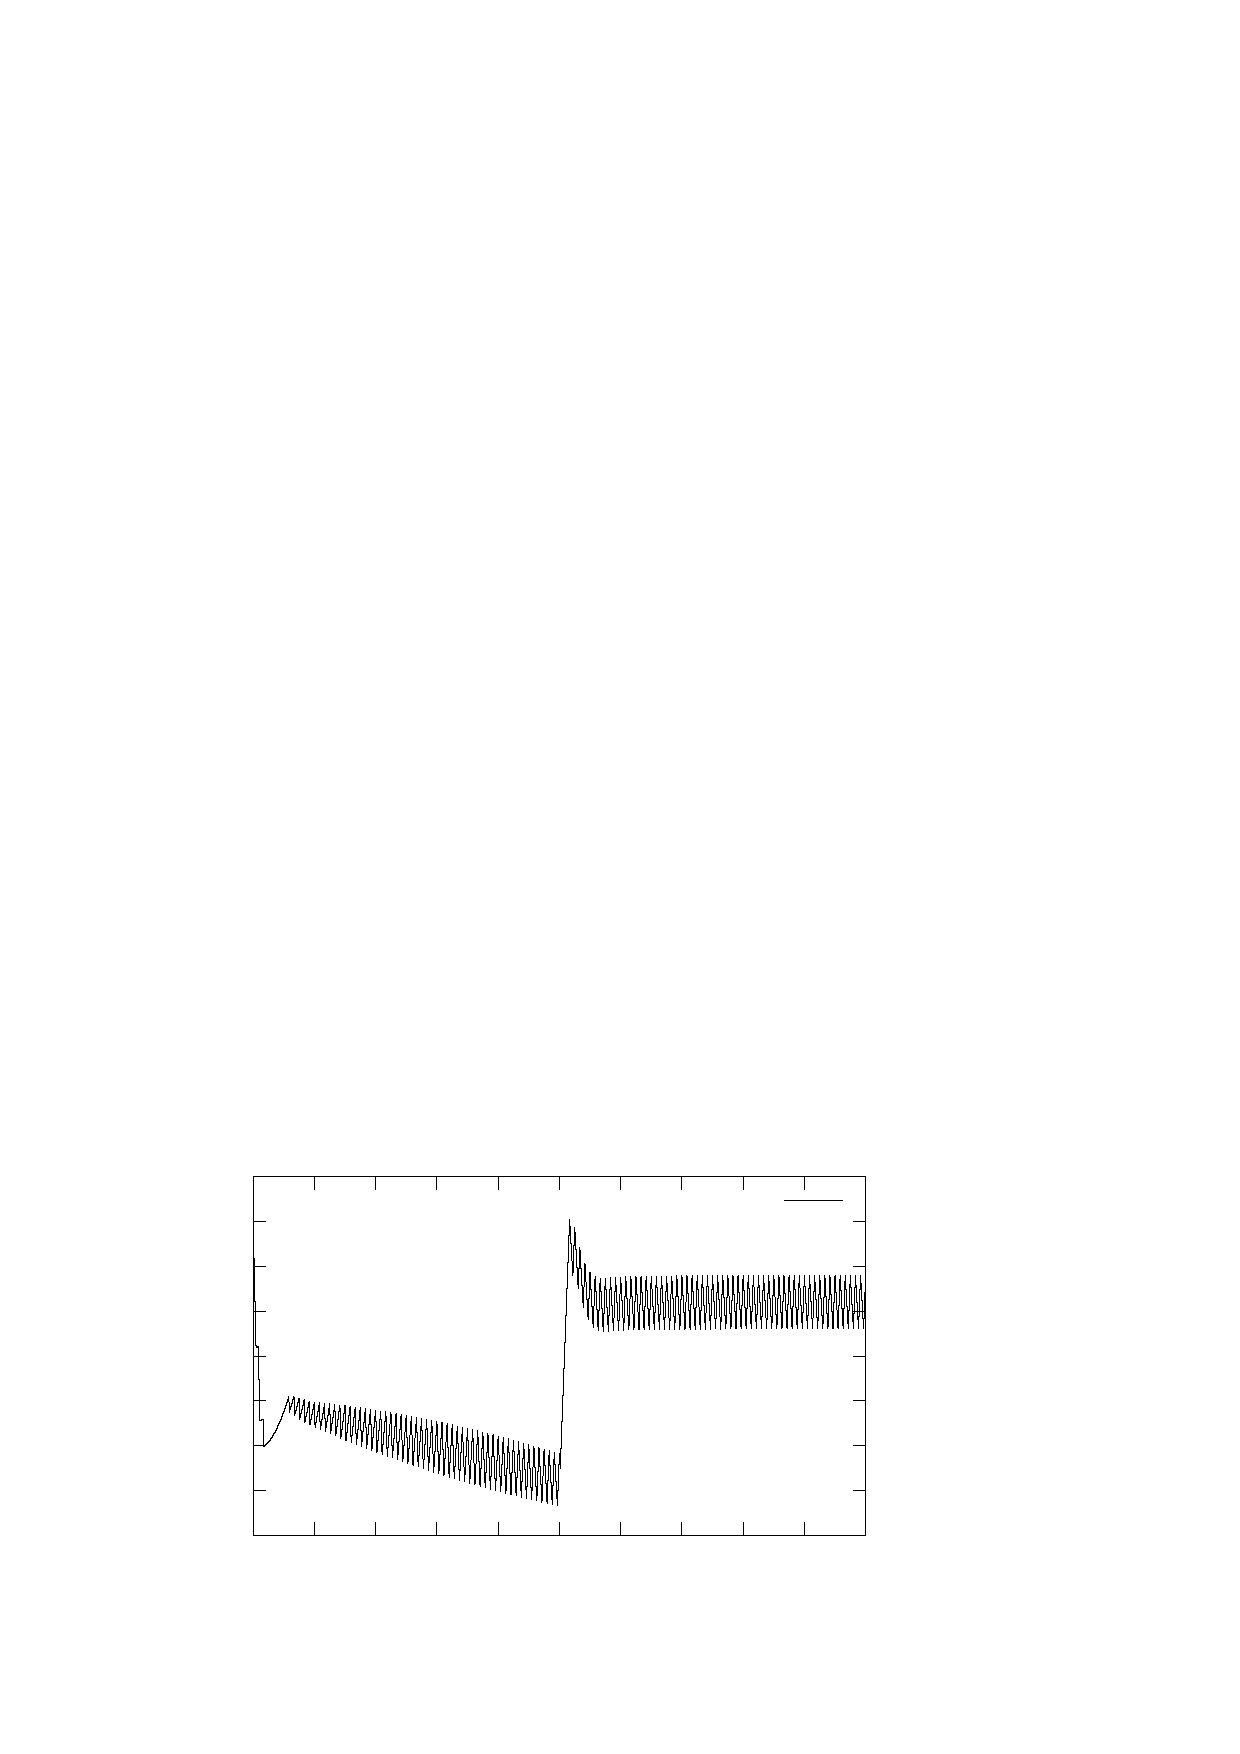
\includegraphics{Buck}%
\end{picture}%
\begingroup
\setlength{\unitlength}{0.0200bp}%
\begin{picture}(18000,10800)(0,0)%
\put(2200,1650){\makebox(0,0)[r]{\strut{}-0.7}}%
\put(2200,2725){\makebox(0,0)[r]{\strut{}-0.6}}%
\put(2200,3800){\makebox(0,0)[r]{\strut{}-0.5}}%
\put(2200,4875){\makebox(0,0)[r]{\strut{}-0.4}}%
\put(2200,5950){\makebox(0,0)[r]{\strut{}-0.3}}%
\put(2200,7025){\makebox(0,0)[r]{\strut{}-0.2}}%
\put(2200,8100){\makebox(0,0)[r]{\strut{}-0.1}}%
\put(2200,9175){\makebox(0,0)[r]{\strut{} 0}}%
\put(2200,10250){\makebox(0,0)[r]{\strut{} 0.1}}%
\put(2475,1100){\makebox(0,0){\strut{}   0}}%
\put(3945,1100){\makebox(0,0){\strut{}   2e-5}}%
\put(5415,1100){\makebox(0,0){\strut{}   4e-5}}%
\put(6885,1100){\makebox(0,0){\strut{}   6e-5}}%
\put(8355,1100){\makebox(0,0){\strut{}   8e-5}}%
\put(9825,1100){\makebox(0,0){\strut{}   1e-4}}%
\put(11295,1100){\makebox(0,0){\strut{}   1.2e-4}}%
\put(12765,1100){\makebox(0,0){\strut{}   1.4e-4}}%
\put(14235,1100){\makebox(0,0){\strut{}   1.6e-4}}%
\put(15705,1100){\makebox(0,0){\strut{}   1.8e-4}}%
\put(17175,1100){\makebox(0,0){\strut{}   2e-4}}%
\put(550,5950){\rotatebox{90}{\makebox(0,0){\strut{}Inductor current}}}%
\put(9825,275){\makebox(0,0){\strut{}time s}}%
\end{picture}%
\endgroup
\endinput

\caption{Buck simulation}
\label{fig-Buck-sim}
\end {figure} 
\newpage
%*************************************OTHER ANALYSIS

%EXAMPLE SECTION************************************************************************************
\section{The Diodes bridge example}

\begin{figure}[h]
\centerline{
 \scalebox{0.7}{
    \input{Bridge.pstex_t}
 }
}
 \caption{Diodes bridge}
\label{fig-Diode-bridge}
\end{figure}




\subsection{Unknowns}

x = $^{t}(U_{1},I_{7})$,
$Z_{ns}=^{t}(I_{2},I_{3},I_{4},I_{5}$),
$Z_{s} = ^{t}(V_{2},V_{3})$
\subsection{Diode non smooth model instance}

\[ \beta = z_{i} = I_{i}\]
\[ \alpha =U_{i}\]
\[z_{i}=1l_{i}+0\alpha\]
\[y_{i}=1\alpha+0l_{i}\]
\[0 \leq y_{i} \, \perp \, l_{i} \geq 0\]


\subsection{Global formulation}

\[ \lambda =(l_{1},l_{2},l_{3},l_{4})\]
\[Z_{ns}=0X+0Z_{s}+Id\lambda\]
\[Y=\left(\begin{array}{cc}
0&0\\
0&0\\
1&0\\
1&0\end{array}\right) x+
\left(\begin{array}{cc}
1&0\\
0&1\\
0&-1\\
-1&0\end{array}
\right) Z_{s} + 0Z_{ns} +0\lambda\]

\[0 \leq Y \, \perp \, \lambda \geq 0\]



\subsection{Matrices formulation}
\[
\left(\begin{array}{c}
  
x'=\left(\begin{array}{cc}
0 &\frac{-1}{C}\\
\frac{1}{L}&0\end{array} \right)x
+\left(\begin{array}{cc}
0&\frac{-1}{C}\\
0&0\end{array} \right)Z_{s}
+\left(\begin{array}{cccc}
0&0&\frac{1}{C}&\frac{-1}{C}\\
0&0&0&0\end{array} \right)Z_{ns}
\\
0=\left(\begin{array}{cc}
0 &0\\
0 &0\\
0 &1\end{array} \right)x
+\left(\begin{array}{cc}
\frac{-1}{R}&\frac{1}{R}\\
\frac{-1}{R}&\frac{1}{R}\\
1&0\end{array} \right)Z_{s}
+\left(\begin{array}{cccc}
1&0&0&1\\
0&+1&1&0\\
0&0&0&0\end{array} \right)Z_{ns}
\\
Z_{ns}=Dx+0Z_{s}+Id\lambda\\
Y=\left(\begin{array}{cc}
0&0\\
0&0\\
1&0\\
1&0\end{array}\right) x+
\left(\begin{array}{cc}
1&0\\
0&1\\
0&-1\\
-1&0\end{array}
\right) Z_{s} + 0Z_{ns} +0\lambda\\

0 \leq Y \, \perp \, \lambda \geq 0

\end{array}
\right)
\]

\subsection{Simulation}
C= 1 uF\\
L= 10 mH\\
R= 1000 $\ohm$\\
The simulation computed 450 steps with a 10 $\micro$s fixed time step. The figure
\ref{fig-Diode-sim} shows the tension in the resistor branch.


\begin {figure}[h]
%GNUPLOT: LaTeX picture with Postscript
\begin{picture}(0,0)%
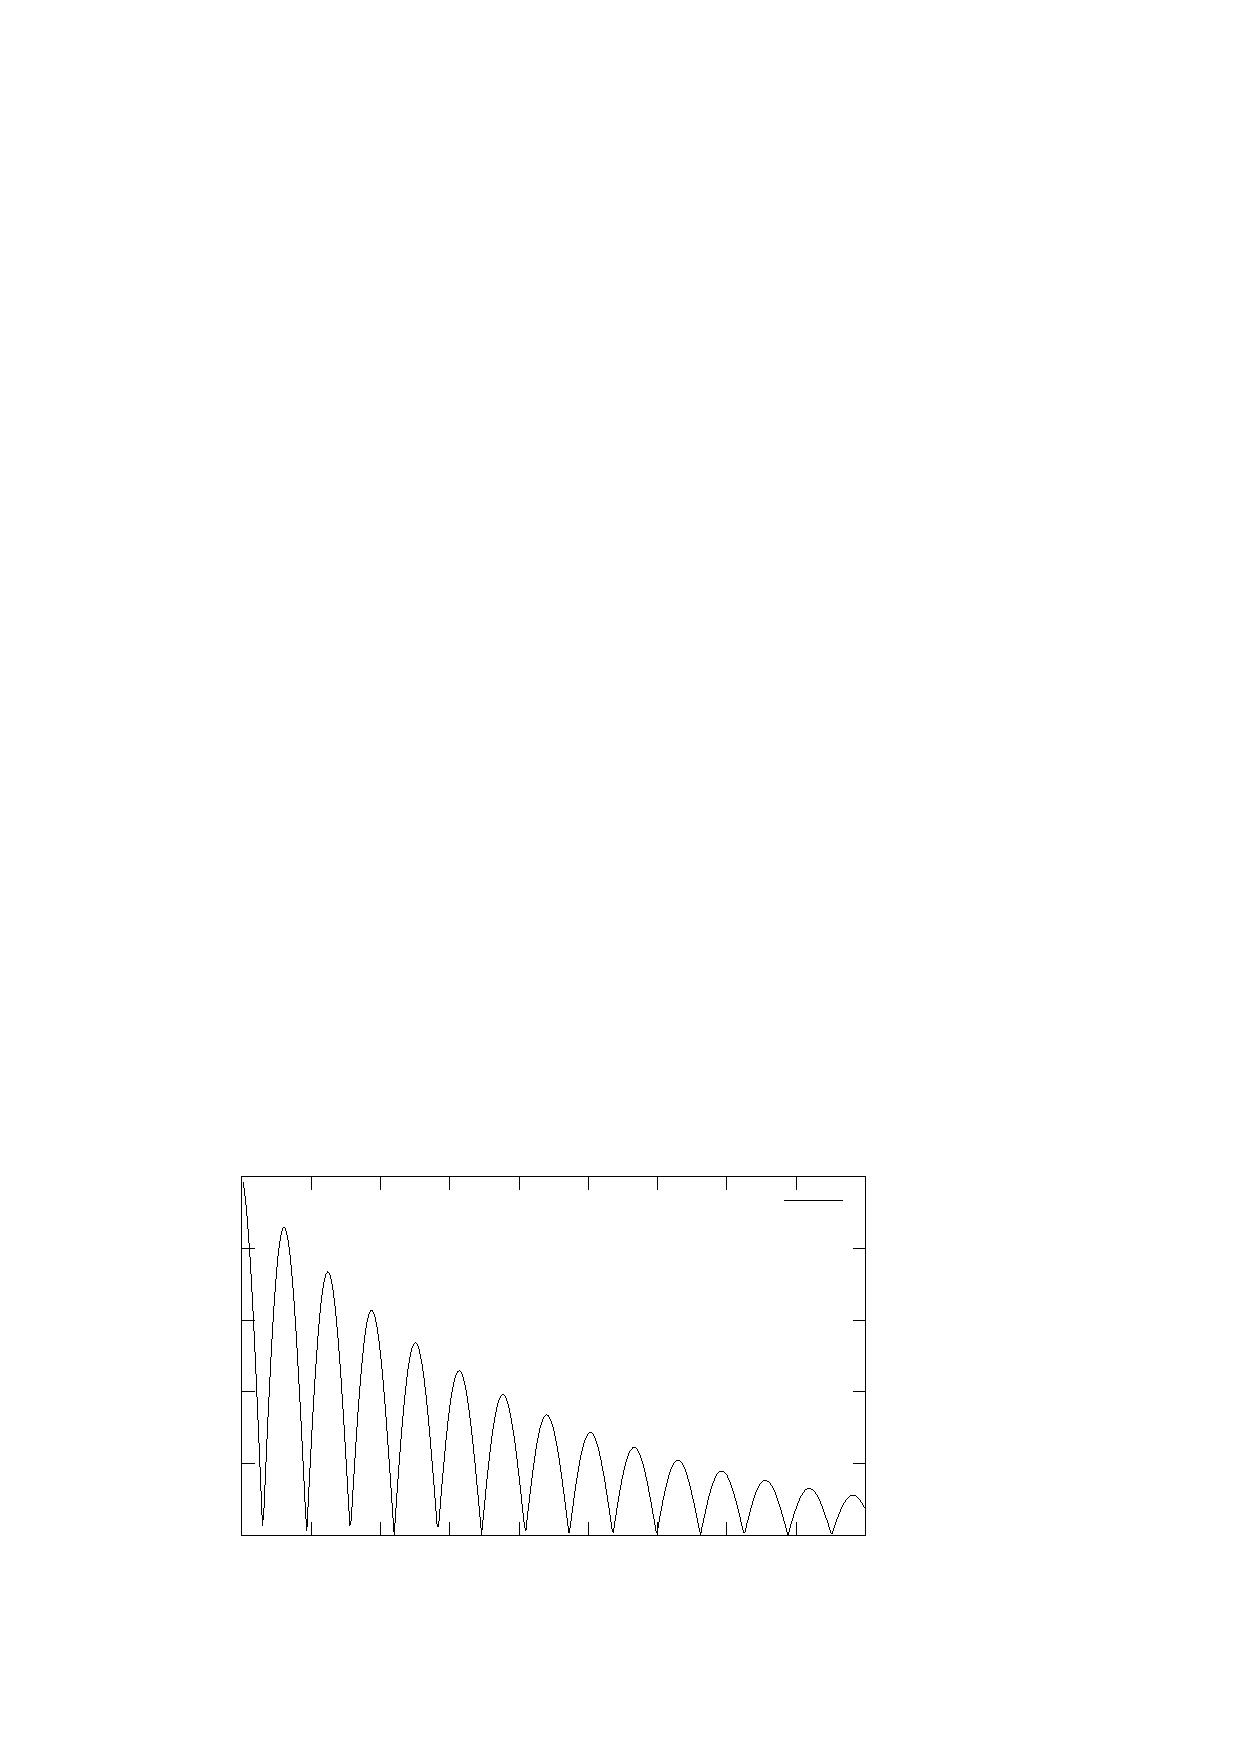
\includegraphics{diodes}%
\end{picture}%
\begingroup
\setlength{\unitlength}{0.0200bp}%
\begin{picture}(18000,10800)(0,0)%
\put(1925,1650){\makebox(0,0)[r]{\strut{} 0}}%
\put(1925,3370){\makebox(0,0)[r]{\strut{} 2}}%
\put(1925,5090){\makebox(0,0)[r]{\strut{} 4}}%
\put(1925,6810){\makebox(0,0)[r]{\strut{} 6}}%
\put(1925,8530){\makebox(0,0)[r]{\strut{} 8}}%
\put(1925,10250){\makebox(0,0)[r]{\strut{} 10}}%
\put(2200,1100){\makebox(0,0){\strut{} 0}}%
\put(3864,1100){\makebox(0,0){\strut{} 50}}%
\put(5528,1100){\makebox(0,0){\strut{} 100}}%
\put(7192,1100){\makebox(0,0){\strut{} 150}}%
\put(8856,1100){\makebox(0,0){\strut{} 200}}%
\put(10519,1100){\makebox(0,0){\strut{} 250}}%
\put(12183,1100){\makebox(0,0){\strut{} 300}}%
\put(13847,1100){\makebox(0,0){\strut{} 350}}%
\put(15511,1100){\makebox(0,0){\strut{} 400}}%
\put(17175,1100){\makebox(0,0){\strut{} 450}}%
\put(550,5950){\rotatebox{90}{\makebox(0,0){\strut{}U23}}}%
\put(9687,275){\makebox(0,0){\strut{}time e-5 s}}%
\put(14950,9675){\makebox(0,0)[r]{\strut{}'DiodeBridge.traj'}}%
\end{picture}%
\endgroup
\endinput

\caption{Diode bridges simulation}
\label{fig-Diode-sim}
\end {figure} 
\section {Cost of the automatic circuit equation formulation}
To evaluate the cost of the automatic circuit equation, we define the following notation:\\
$N_{b}$ is the number of branches.\\
$N_{n}$ is the number of nodes. ( $N_{n} < 2N_{b}$ )\\
N = max\{$N_{b},N_{n}$\}\\
dim(x) is the number of dynamical variables.\\
\\
The costs of the main steps are:\\

\begin{itemize}

\item[--]To parse the Netlist : \\It consists in reading and storing the Netlist. The cost is O(N).
\item[--] To build the unknowns vector:\\
O(N) operations are necessary to build the vector with voltage nodes.\\
Each components add its own unknowns, it costs O(N).
\item[--] To get the system $x' = A_{1x}x +A_{1zs}Z_{s} + A_{1ns}Z_{ns}+A_{1s}$:\\
The Minimum Spanning Tree algorithm complexity is O(Nlog(N))\\
To reverse the matrix A with a LU factorization: O$(dim(x))^{3}$
\item[--] Stamping method:\\
Each component writes its contribution in the table equation, it costs O(N).
\item[--] Matrix product:\\
Multiplied two dense matrices costs O($N^{3}$). In our case, the matrices are very sparse. So
the cost is considerably reduced with a sparse matrices structure.

\end{itemize}
For example, the automatic circuit equation formulation of the buck converter needs 0.012 s on a Pentium~4 processor clocked at 3~GHz.

\section{Conclusion}
This document demonstrates a way to develop an automatic circuit equation formulation. It shows that a Moreau's time
stepping lead to a MLCP. The previous examples describe the method with non smooth circuits.


%%% Local Variables: 
%%% mode: latex
%%% TeX-master: "ace"
%%% End: 
